\documentclass[cjk,slidestop,compress,mathserif,blue]{beamer}
%dvipdfm选项是关键,否则编译统统通不过
%beamer的颜色选项定义的是导航条和标题的颜色(即关键词structure的颜色)

%%%%%%%%%%%%%%%%仅限于XeTeX可使用的宏包%%%%%%%%%%%%%%%%%%%%%%%%%%%%
\usepackage{fontspec,xunicode,xltxtra,beamerthemesplit}
%\usepackage{beamerthemesplit}
\usepackage{handoutWithNotes}		%(讲义)在打印PPT的时候会留出给每一页做注释的部分
\usepackage{xeCJK}
\setCJKmainfont[BoldFont=黑体, ItalicFont=楷体, BoldItalicFont=仿宋]{黑体}
%\setsansfont[Mapping=tex-text]{Adobe 黑体 Std}
%如果装了Adobe Acrobat,可在font.conf中配置Adobe字体的路径以使用其中文字体
%也可直接使用系统中的中文字体如SimSun,SimHei,微软雅黑 等
%原来beamer用的字体是sans family;注意Mapping的大小写,不能写错

\usepackage{listings} 
\lstset{language=Matlab}%代码语言使用的是matlab 
\lstset{breaklines}%自动将长的代码行换行排版 
\lstset{extendedchars=false}%解决代码跨页时,章节标\dots

%%%%%%%%   确定标题和导航条结构的框架     %%%%%%%%%%%%
\usepackage{beamerthemeshadow}                       %
%\usepackage{beamerthemeclassic}%导航条色与背景色一致%
%%%%%%%%%%%%%%%%%%%%%%%%%%%%%%%%%%%%%%%%%%%%%%%%%%%%%%
\setbeamerfont{roman title}{size={}}
%\usepackage{CJK} % CJK 中文支持                                  %
\usepackage{amsmath,amsthm,amsfonts,amssymb,bm}
\usepackage{mathrsfs}
\usepackage{xcolor}                                        %使用默认允许使用颜色
\usepackage{hyperref} 
\usepackage{graphicx}
\usepackage{subfigure}           %图片跨页
\usepackage{animate}		 %插入动画
\usepackage{caption}
\captionsetup{font=footnotesize}

\usepackage{multirow}

\usepackage[dvipdfmx]{movie15_dvipdfmx} %插入视频
%\usepackage{handoutWithNotes}		%(讲义)在打印PPT的时候会留出给每一页做注释的部分
%\pgfpagesuselayout{1 on 1 with notes landscape}[a4paper,border shrink=5mm]

%\usepackage[numbers,sort&compress]{natbib} %紧密排列             %
\usepackage[sectionbib]{chapterbib}        %每章节单独参考文献   %
\usepackage{hypernat}                                                                         %
%\usepackage[dvipdfm,bookmarksopen=true,pdfstartview=FitH,CJKbookmarks]{hyperref}		%
\hypersetup{bookmarksnumbered,colorlinks,linkcolor=brown,citecolor=blue,urlcolor=red}         %
%参考文献含有超链接引用时需要下列宏包,注意与natbib有冲突        %
%\usepackage[dvipdfm]{hyperref}                                  %
%\usepackage{hypernat}                                           %
\newcommand{\upcite}[1]{\hspace{0ex}\textsuperscript{\cite{#1}}} %

%\usepackage{marvosym} %插入各种符号

%\useoutertheme{smoothbars}
\useinnertheme[shadow=true]{rounded}
\usetheme{Berkeley}                                          %主题式样
%\usetheme{Luebeck}

\usecolortheme{lily}                                        %颜色主题式样

\usefonttheme{professionalfonts}                           %字体主题样式宏包

%\beamertemplatetransparentcoveredhigh                      %使所有被隐藏的文本高度透明
\beamertemplatetransparentcovereddynamicmedium             %使所有被隐藏的文本完全透明,动态,动态的范围很小
\mode<presentation>
%\beamersetaveragebackground{gray}                          %设置背景颜色(单一色) 
\beamertemplateshadingbackground{green!10}{red!5}         %设置背景颜色(渐变色)

%i放置单位logo
%\logo{
\includegraphics[width=1.6cm,height=0.35cm]{Figures/BCC_logo-1.png}}	%简单设置logo

%\pgfdeclareimage[width=3.5cm]{logoname}{Figures/BCC_logo-1.png}		%logo置于左侧微调
%\logo{\pgfuseimage{logoname}{\vspace{0.2cm}\hspace*{-2.0cm}}}

%在指定位置精确放置logo
\usepackage{tikz}
\usepackage{beamerfoils}
\usepackage{pgf}
\logo{\pgfputat{\pgfxy(11.68,0.15)}{
\includegraphics[height=1.01cm,viewport=0 0 140 120,clip]{Figures/BCC_logo-1.png}}\pgfputat{\pgfxy(10.502,-0.218)}{
\includegraphics[height=0.369cm,viewport=140 0 540 120,clip]{Figures/BCC_logo-1.png}}}
%\logo{\pgfputat{\pgfxy(11.68,0.15)}{
\includegraphics[height=0.95cm,viewport=0 0 510 360,clip]{Figures/Logo_Gainstrong.png}}\pgfputat{\pgfxy(10.333,-0.195)}{
\includegraphics[height=0.35cm,viewport=530 70 1100 218,clip]{Figures/Logo_Gainstrong.png}}}
%\logo{\pgfputat{\pgfxy(10.28,0.00)}{
\includegraphics[height=0.95cm,viewport=0 0 1100 360,clip]{Figures/Logo_Gainstrong.png}}}
%\logo{\pgfputat{\pgfxy(11.68,0.15)}{
\includegraphics[height=0.95cm,viewport=0 0 510 360,clip]{Figures/Logo_Gainstrong.png}}\pgfputat{\pgfxy(10.333,-0.195)}{
\includegraphics[height=0.35cm,viewport=530 70 1100 218,clip]{Figures/Logo_Gainstrong.png}}}
%\MyLogo{
%	\pgfputat{\pgfxy(-50,-50)}{\pgfbox[right,base]{
\includegraphics[height=1cm]{Figures/BCC_logo-1.png}}}

%logo作为背景放置
%\setbeamertemplate{background}{
%	\pgfputat{\pgfxy(6.5,-0.5)}{\pgfbox[left,top]{\pgfimage[height=1.1cm]{Figures/BCC_logo-1.png}}}}

%\logo{}									%不显示logo

\begin{document}
%\begin{CJK*}{GBK}{song}
%\begin{CJK*}{GBK}{kai}
%beamer下不能用\songyi、\zihao等命令!
%\graphicspath{Figures/}

%-------------------------------PPT Title-------------------------------------
\title{\rm{VASP~}的输入文件\rm{INCAR~}参数简介}
%-----------------------------------------------------------------------------

%----------------------------Author & Date------------------------------------
\author[\textrm{Jun\_Jiang}]{姜\;\;骏\inst{}} %[]{} (optional, use only with lots of authors)
% - Give the names in the same order as the appear in the paper.
% - Use the \inst{?} command only if the authors have different
%   affiliation.
\institute[BCC]{\inst{}%
 \vskip -30pt 北京市计算中心}
\date[\today] % (optional, should be abbreviation of conference name)
{	{\fontsize{6.2pt}{4.2pt}\selectfont{\textcolor{blue}{E-mail:~}\url{jiangjun@bcc.ac.cn}}}
\vskip 45 pt 2019.04.07
\vskip 5 pt {\fontsize{8.2pt}{6.2pt}\selectfont{清华大学\;\;物理系}}}

% - Either use conference name or its abbreviation
% - Not really information to the audience, more for people (including
%   yourself) who are reading the slides online

\subject{}
% This is only inserted into the PDF information catalog. Can be left
% out.
\frame
{
%	\frametitle{\fontsize{9.5pt}{5.2pt}\selectfont{\textcolor{orange}{“高通量并发式材料计算算法与软件”年度检查}}}
\titlepage
}
%-----------------------------------------------------------------------------

%------------------------------------------------------------------------------列出全文 outline ---------------------------------------------------------------------------------
\section*{}
\frame[allowframebreaks]
{
  \frametitle{Outline}
%  \frametitle{\textcolor{mycolor}{\secname}}
  \tableofcontents%[current,currentsection,currentsubsection]
}
%在每个section之前列出全部Outline
%类似的在每个subsection之前列出全部Outline是\AtBeginSubsection[]
\AtBeginSection[]
{
  \frame<handout:0>
  {
    \frametitle{Outline}
%全部Outline中,本部分加亮
    \tableofcontents[current,currentsection]
  }
}

%------------------------------------------------------------------------------PPT main Body------------------------------------------------------------------------------------
\section{\rm{VASP}~的特点}
\frame
{
	\frametitle{\rm{VASP}~软件的特点}
\begin{figure}[h!]
	\vspace{-0.2in}
\centering

\includegraphics[height=1.2in,width=2.3in,viewport=70 0 800 420,clip]{Figures/Logo_VASP.png}
%\caption{\small \textrm{The Schematic description of the dual grid technique.}}%(与文献\cite{EPJB33-47_2003}图1对比)
\label{VASP_logo}
\end{figure} 
\begin{itemize}
	\item \textrm{PAW}~方法\upcite{PRB59-1758_1999}:\\
		基于\textrm{Ultra-Soft}~赝势的方法\quad{\textcolor{magenta}{主要体现于\textrm{POTCAR}}}
	\item \textrm{Car-Parrinello~}计算技术\upcite{Comp_Phys}:\\
		\textrm{Ab-initio}~分子动力学\quad{\textcolor{magenta}{与传统\textrm{Hamiltonian~}求解差异}}
	\item 优化算法\upcite{CMS6-15_1996,PRB54-11169_1996}:\\
		多种计算参数的控制
\end{itemize}
}

\frame
{
	\frametitle{能量泛函的直接优化}
	根据\textrm{Car-Parrinello~}定义的经典\textrm{Lagrangian~}量
	{\fontsize{9.0pt}{5.2pt}\selectfont
	\begin{displaymath}
		L(\{\psi_k\},\{\vec R_n\})=\frac{\mu}2\sum_k\dot{\psi}_k^2+\sum_n\frac{M_n}2\dot{\vec R}_n^2-E_{\mathrm{tot}}(\{\psi_k\},\{\vec R_n\})+\sum_{kl}\Lambda_{kl}\langle\psi_k|\psi_l\rangle
	\end{displaymath}}
	多粒子体系的\textrm{Euler-Lagrange~}运动方程可以表示为
	\begin{displaymath}
		\begin{aligned}
			\mu\ddot{\psi}_k=&-\dfrac{\partial E_{\mathrm{tot}}}{\partial\psi_k}+2\sum_i\Lambda_{kl}\psi_l(\vec r)\\
			M_n\ddot{\vec R}_n&=-\dfrac{\partial E_{\mathrm{tot}}}{\partial\vec R_n}+\sum_{kl}\Lambda_{kl}\dfrac{\partial\langle\psi_k|\psi_l\rangle}{\partial\vec R_n}
		\end{aligned}
	\end{displaymath}
	\textcolor{purple}{电子基态可以通过求解\textrm{Verlet~}运动方程得到}\\
	在\textrm{DFT~}框架下,有
	{\fontsize{9.0pt}{5.2pt}\selectfont
	\begin{displaymath}
		\psi_k(t+h)=2\psi_k(t)-\psi_k(t-h)-\dfrac{2h^2}{\mu}(H\psi_k-\sum_l\Lambda_{kl}\psi_l)
	\end{displaymath}}
%	该方程表明:~\textcolor{blue}{电子基态也可通过各种优化方法直接求解}
	每个时间步$t$,\textrm{Car-Parrinello~}采用变分法迭代确定$\psi_k(t)$
}

\frame
{
	\frametitle{计算流程}
\begin{figure}[h!]
	\vspace{-0.2in}
\centering
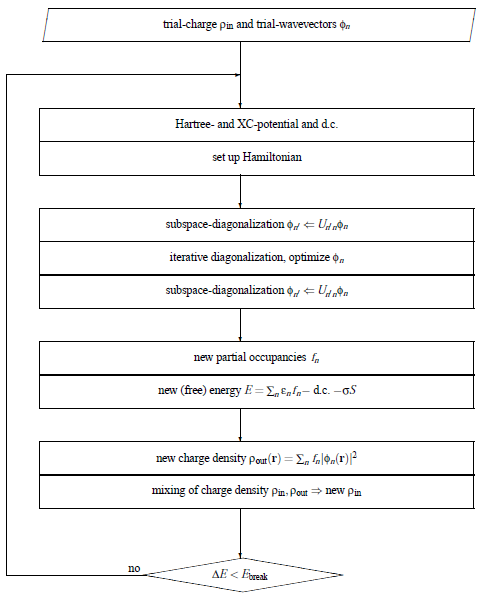
\includegraphics[height=2.1in,width=1.6in,viewport=0 0 480 630,clip]{Figures/VASP_procedure.png}
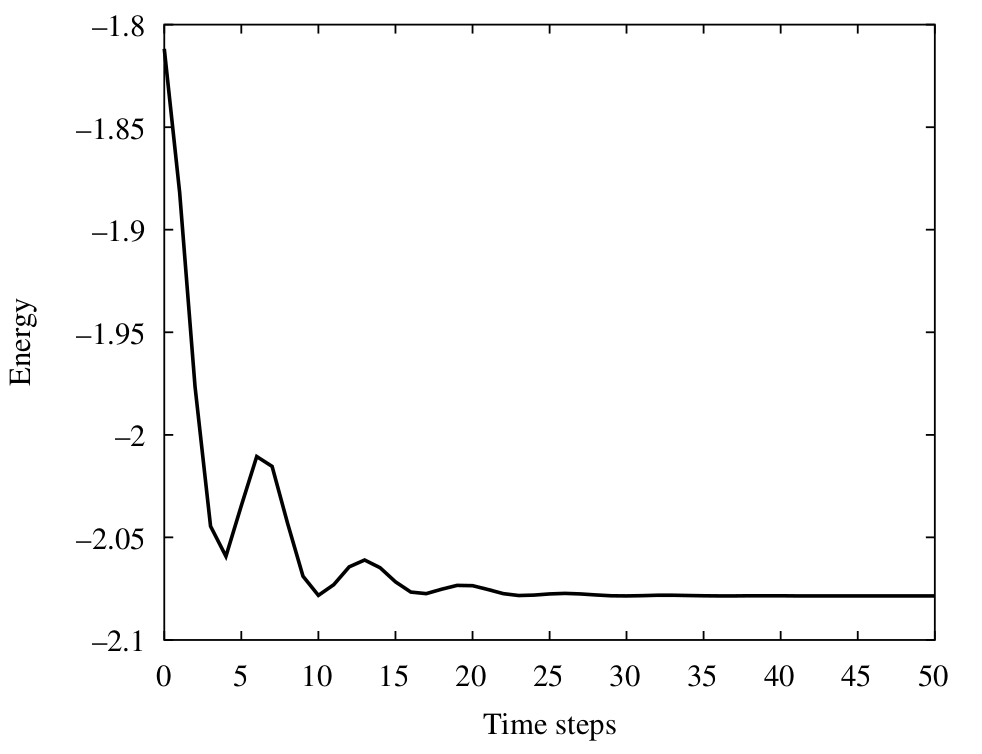
\includegraphics[height=2.1in,width=2.3in,viewport=0 0 740 600,clip]{Figures/Ab-initio-Ene.png}
\caption{\small \textrm{The Flow of calculation for the KS-ground states.}}%(与文献\cite{EPJB33-47_2003}图1对比)
\label{PAW_baiseset}
\end{figure} 
}

\subsection{方程迭代求解与函数优化基本思想}
\frame
{
	\frametitle{非线性方程的\rm{Newton~}法求根}
	\textcolor{blue}{不管哪一种数值算法,其设计原理都是将复杂转化为简单的重复,或者说,通过简单的重复生成复杂}:\\\textcolor{red}{在算法设计和算法实现过程中,重复就是力量}
\begin{figure}[h!]
\centering
\animategraphics[autoplay, loop, height=2.1in]{1}{Figures/OP_Newton_}{0}{17}
\label{Equation_Newon}
\end{figure}
}

\section{\rm{INCAR}~主要输入参数分类}
\subsection{计算量控制参数}
\frame
{
\frametitle{主要输入参数}
\begin{enumerate}
	\item \textcolor{red}{Dimension of arrays:}
	\begin{itemize}
		\item \textcolor{blue}{NKPTS} = 16~~\textcolor{brown}{\fontsize{9.2pt}{3.9pt}\selectfont{k-points}}\\
		\textcolor{blue}{NKDIM} = 16~~\textcolor{brown}{\fontsize{9.2pt}{3.9pt}\selectfont{k-points in BZ}}
		\item \textcolor{blue}{NBANDS}= 5~~\textcolor{brown}{\fontsize{9.2pt}{3.9pt}\selectfont{number of bands}}
		\item \textcolor{blue}{NEDOS} = 301~~\textcolor{brown}{\fontsize{9.2pt}{3.9pt}\selectfont{number of dos}}
		\item \textcolor{blue}{NIONS} = 1~~\textcolor{brown}{\fontsize{9.2pt}{3.9pt}\selectfont{number of ions}}\\
		\textcolor{blue}{ions per type}        =      1
		\item \textcolor{blue}{LDIM}  = 4~~\textcolor{brown}{\fontsize{9.2pt}{3.9pt}\selectfont{non local maximal}}\\
		\textcolor{blue}{LMDIM} = 8~~\textcolor{brown}{\fontsize{9.2pt}{3.9pt}\selectfont{non local SUM 2l+1}}
		\item \textcolor{blue}{NPLWV} = 1000~~\textcolor{brown}{\fontsize{9.2pt}{3.9pt}\selectfont{total plane-waves}}
		\item \textcolor{blue}{IRMAX} = 1~~\textcolor{brown}{\fontsize{9.2pt}{3.9pt}\selectfont{max r-space proj}}
		\item \textcolor{blue}{IRDMAX}= 2458~~\textcolor{brown}{\fontsize{9.2pt}{3.9pt}\selectfont{max aug-charges}}
		\item \textcolor{magenta}{NGX} =  10~~\textcolor{magenta}{NGY} = 10~~\textcolor{magenta}{NGZ} = 10~~\textcolor{brown}{\fontsize{9.2pt}{3.9pt}\selectfont{dimension x,y,z}}\\
		\textcolor{magenta}{NGXF}= 20~~\textcolor{magenta}{NGYF}= 20~~\textcolor{magenta}{NGZF}= 20~~\textcolor{brown}{\fontsize{9.2pt}{3.9pt}\selectfont{dimension x,y,z}}\\
		\textcolor{magenta}{NGXF}= 20~~\textcolor{magenta}{NGYF}= 20~~\textcolor{magenta}{NGZF}= 20~~\textcolor{brown}{\fontsize{9.2pt}{3.9pt}\selectfont{support grid}}
	\end{itemize}
\end{enumerate}
}

\frame
{
	\frametitle{双网格技术}
\begin{figure}[h!]
	\vspace{-0.2in}
\centering
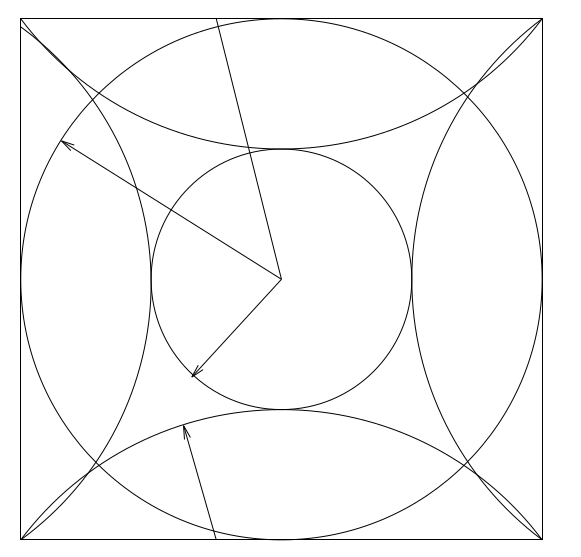
\includegraphics[height=2.3in,width=2.3in,viewport=0 0 420 420,clip]{Figures/VASP_G_max.png}
\caption{\fontsize{5.2pt}{3.9pt}\selectfont{\textrm{The small sphere contains all plane waves included in the basis set $\vec G<\vec G_\mathrm{cut}$. The charge density contains components up to $2\vec G$ cut (second sphere), and the acceleration a components up to $3\vec G$ cut , which are reflected in (third sphere) because of the finite size of the FFT-mesh. Nevertheless the components a $\vec G$ with $|\vec G|<\vec G$ cut are correct i.e. the small sphere does not intersect with the third large sphere. Fig. from \cite{VASP_UG}}}}%(与文献\cite{EPJB33-47_2003}图1对比)
\label{VASP_G_max}
\end{figure} 
}

\frame
{
	\frametitle{双网格技术}
\begin{figure}[h!]
	\vspace{-0.2in}
\centering
%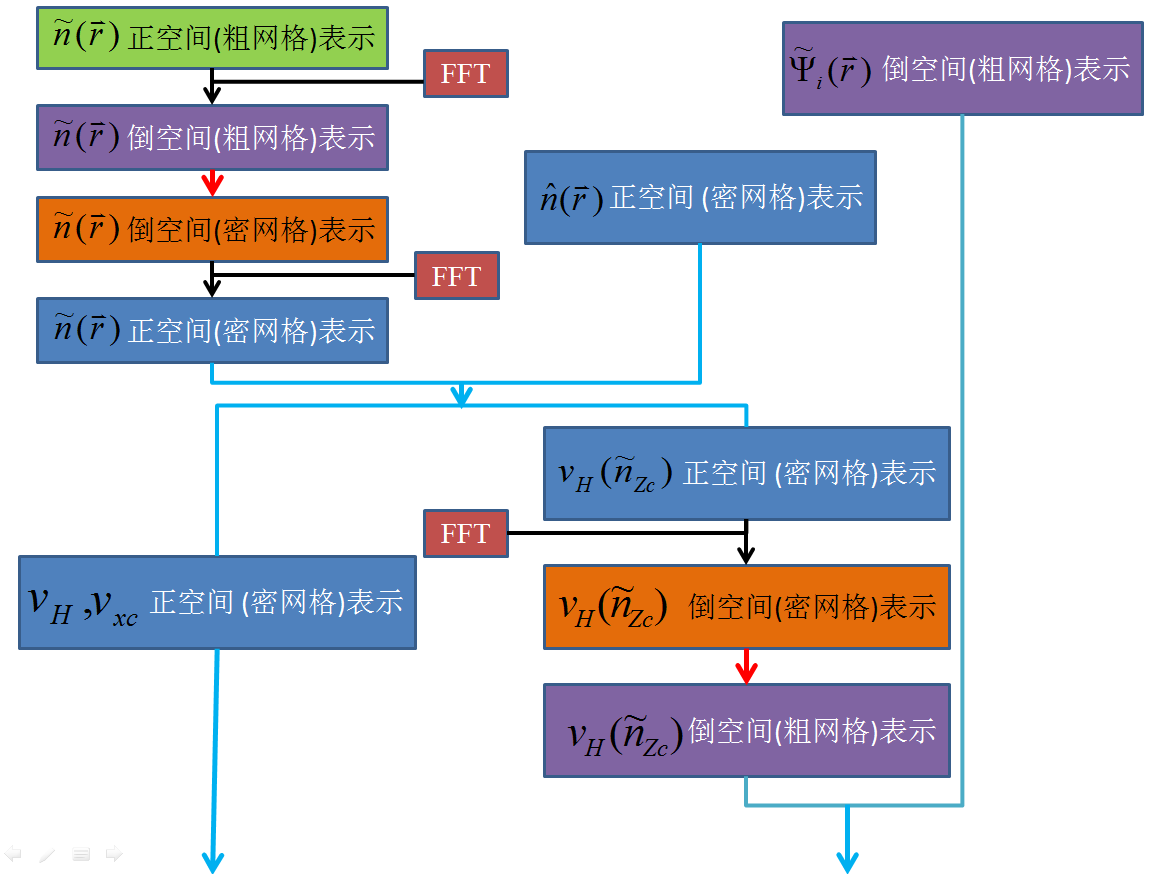
\includegraphics[height=2.7in,width=4.0in,viewport=0 0 1180 875,clip]{Figures/dual_grid.png}
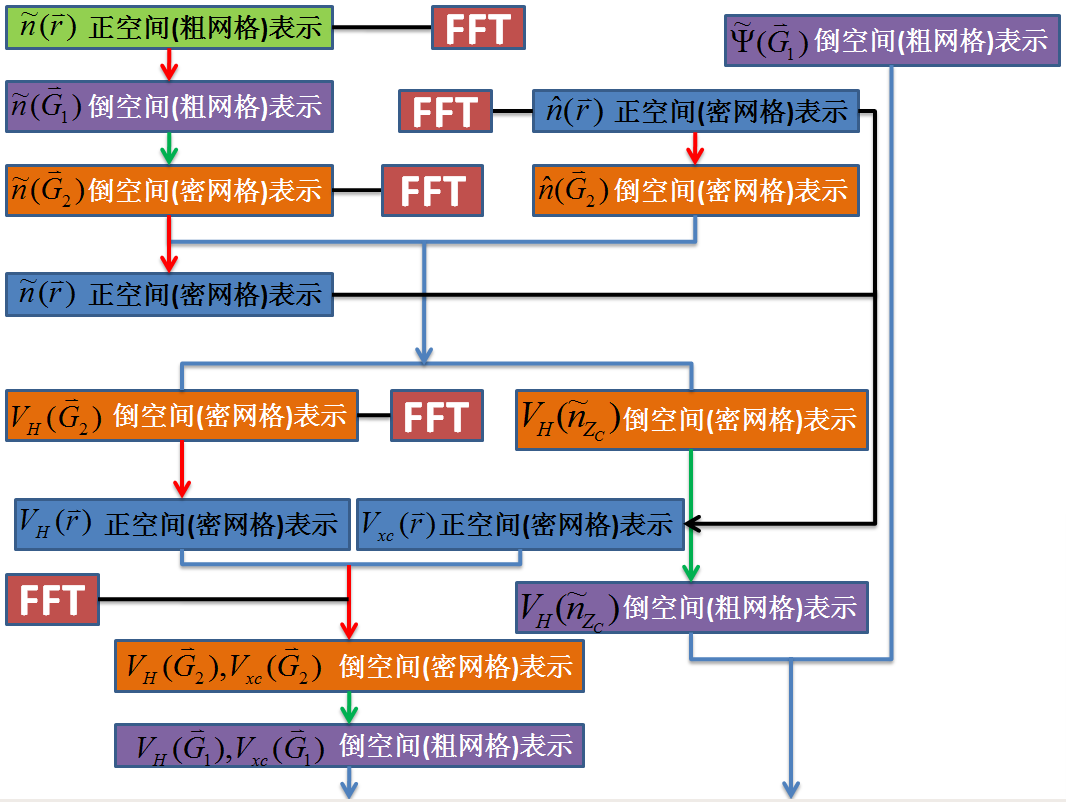
\includegraphics[height=2.7in,width=4.0in,viewport=0 0 800 600,clip]{Figures/dual_grid-2.png}
\caption{\small \textrm{The Schematic description of the dual grid technique.}}%(与文献\cite{EPJB33-47_2003}图1对比)
\label{PAW_baiseset}
\end{figure} 
}

\frame
{
\frametitle{主要输入参数}
\begin{description}
	\item[\textcolor{blue}{POSCAR}]=  FCC-Al~~\textcolor{brown}{\fontsize{9.2pt}{3.9pt}\selectfont{\# comment line}} 
	\item[\textcolor{blue}{SYSTEM}]=  Al: fcc                                 
	\item[] \textcolor{magenta}{I would recommend the setting:}
	\item[\textcolor{blue}{NGX}] = 10~~\textcolor{blue}{NGY} = 10~~\textcolor{blue}{NGZ} = 10~~\textcolor{brown}{\fontsize{7.2pt}{3.9pt}\selectfont{dimension x,y,z}}
\end{description}
}

\subsection{计算过程控制参数}
\frame
{
\frametitle{主要输入参数}
\begin{enumerate}
\setcounter{enumi}{1}
	\item \textcolor{red}{\textrm{Startparameter for this run:}}
		\begin{description}
			\item[\textcolor{blue}{NWRITE}] = 2~~\textcolor{brown}{\fontsize{9.2pt}{3.9pt}\selectfont{write-flag \& timer}}\\

			\item[\textcolor{blue}{PREC}]   = normal~~\textcolor{brown}{\fontsize{9.2pt}{3.9pt}\selectfont{normal or accurate \textcolor{magenta}{(medium, high low for compatibility)}}}
			\item[\textcolor{blue}{ISTART}] = 1~~\textcolor{brown}{\fontsize{9.2pt}{3.9pt}\selectfont{job :~\textcolor{magenta}{0-new  1-cont  2-samecut}}}\\

			\item[\textcolor{blue}{ICHARG}] = 1 ~~\textcolor{brown}{\fontsize{9.2pt}{3.9pt}\selectfont{charge:~\textcolor{magenta}{1-file 2-atom 10-const}}}\\

			\item[\textcolor{blue}{ISPIN}]  = 1 ~~\textcolor{brown}{\fontsize{9.2pt}{3.9pt}\selectfont{spin polarized calculation?}}\\

			\item[\textcolor{blue}{LNONCOLLINEAR}] = F ~~\textcolor{brown}{\fontsize{9.2pt}{3.9pt}\selectfont{non collinear calculations}}\\

			\item[\textcolor{blue}{LSORBIT}] = F ~~\textcolor{brown}{\fontsize{9.2pt}{3.9pt}\selectfont{spin-orbit coupling}}\\

			\item[\textcolor{blue}{INIWAV}] =  1 ~~\textcolor{brown}{\fontsize{9.2pt}{3.9pt}\selectfont{electr:~\textcolor{magenta}{0-lowe 1-rand  2-diag}}}\\

			\item[\textcolor{blue}{LASPH}]  =  F ~~\textcolor{brown}{\fontsize{9.2pt}{3.9pt}\selectfont{aspherical Exc in radial PAW}}\\

			\item[\textcolor{blue}{METAGGA}]=  F ~~\textcolor{brown}{\fontsize{9.2pt}{3.9pt}\selectfont{non-selfconsistent MetaGGA calc.}}
		\end{description}
\end{enumerate}
}

\subsection{离子-分子动力学计算控制参数}
\frame
{
\frametitle{主要输入参数}
\begin{enumerate}
\setcounter{enumi}{2}
 \item \textcolor{red}{\textrm{Ionic relaxation}}
	 \begin{description}
		 \item[\textcolor{blue}{EDIFFG}] = 0.1E-02 ~~\textcolor{brown}{\fontsize{9.2pt}{3.9pt}\selectfont{stopping-criterion for IOM}}
		 \item[\textcolor{blue}{NSW}] =      0 ~~\textcolor{brown}{\fontsize{9.2pt}{3.9pt}\selectfont{number of steps for IOM}}
		 \item[\textcolor{blue}{NBLOCK}] = 1; \textcolor{blue}{KBLOCK} = 1~~\textcolor{brown}{\fontsize{9.2pt}{3.9pt}\selectfont{inner block; outer block}}
			 \item[\textcolor{red}{IBRION}] = -1~~\textcolor{brown}{\fontsize{9.2pt}{3.9pt}\selectfont{ionic relax: ~\textcolor{magenta}{0-MD 1-quasi-New 2-CG}}}
			 \item[\textcolor{blue}{NFREE}]  = 0~~\textcolor{brown}{\fontsize{8.2pt}{3.9pt}\selectfont{steps in history (QN), initial steepest desc. (CG)}}
			 \item[\textcolor{magenta}{ISIF}]   = 2~~\textcolor{brown}{\fontsize{9.2pt}{3.9pt}\selectfont{stress and relaxation}}
			 \item[\textcolor{blue}{IWAVPR}] =10~~\textcolor{brown}{\fontsize{9.2pt}{3.9pt}\selectfont{prediction: ~\textcolor{magenta}{0-non 1-charg 2-wave 3-comb}}}
			 \item[\textcolor{blue}{ISYM}]   = 2~~\textcolor{brown}{\fontsize{9.2pt}{3.9pt}\selectfont{\textcolor{magenta}{0-nonsym 1-usesym 2-fastsym}}}
			 \item[\textcolor{blue}{LCORR}]  = T~~\textcolor{brown}{\fontsize{9.2pt}{3.9pt}\selectfont{Harris-Foulkes like correction to forces}}
	 \end{description}
\end{enumerate}
}

\frame
{
\frametitle{主要输入参数}
\textcolor{purple}{\textrm{Additional Abinit~MD parameters:~}}
	 \begin{description}
			 \item[\textcolor{magenta}{POTIM}]  = 0.5000 ~~\textcolor{brown}{\fontsize{9.2pt}{3.9pt}\selectfont{time-step for ionic-motion}}
			 \item[\textcolor{blue}{TEIN}]   = 0.0 ~~\textcolor{brown}{\fontsize{9.2pt}{3.9pt}\selectfont{initial temperature}}
			 \item[\textcolor{blue}{TEBEG}]  = 0.0; \textcolor{blue}{TEEND}= 0.0 ~~\textcolor{brown}{\fontsize{9.2pt}{3.9pt}\selectfont{temperature during run}}
			 \item[\textcolor{magenta}{SMASS}]  = -3.00 ~~\textcolor{brown}{\fontsize{9.2pt}{3.9pt}\selectfont{Nose mass-parameter (am)}}
			 \item[\textcolor{blue}{estimated Nose-frequenzy (Omega)}] = 0.10E-29 \\\textcolor{brown}{\fontsize{9.2pt}{3.9pt}\selectfont{period in steps =****** mass=  -0.192E-27a.u.}}
		 \item[\textcolor{blue}{SCALEE}] = 1.0000 ~~\textcolor{brown}{\fontsize{9.2pt}{3.9pt}\selectfont{scale energy and forces}}
		 \item[\textcolor{blue}{NPACO}]  = 256; \textcolor{blue}{APACO}= 16.0 ~~\textcolor{brown}{\fontsize{9.2pt}{3.9pt}\selectfont{distance and # of slots for P.C.}}
		\item[\textcolor{blue}{PSTRESS}]= 0.0 ~~\textcolor{brown}{\fontsize{9.2pt}{3.9pt}\selectfont{pullay stress}}
	 \end{description}
   }

   \frame
   {
	   \frametitle{第一原理-分子动力学中的迭代优化:~离子弛豫}
	\begin{itemize}
		   \item \textrm{quasi-Newton~(RMM-DIIS)}:~\textcolor{blue}{IBRION}=1\\
			
		   \item \textrm{Conjugate-Gradient (CG)}:~\textcolor{blue}{IBRION}=2\\
			
		   \item \textrm{Damping factor($\alpha$=\textcolor{blue}{POTIM};~$\mu$=\textcolor{blue}{SMASS})}\textcolor{blue}{IBRION}=3
			   \begin{displaymath}
				   \begin{aligned}
				   	\ddot{\vec x}&=-2\cdot\alpha\vec F-\mu\dot{\vec x}\\
					\vec v_{\mathrm{N+1/2}}&=\bigg((1-\mu/2)\vec v_{\mathrm{N}-1/2}-2\cdot\alpha\vec F_{\mathrm{N}}\bigg)/(1+\mu/2)\\
					\vec x_{\mathrm{N+1}}&=\vec x_{\mathrm{N}}+\vec v_{\mathrm{N}+1/2}
				   \end{aligned}
			   \end{displaymath}
	\end{itemize}
   }

\frame
{
	\frametitle{迭代优化基本思想}
	对于给定函数$f$,在极值点,函数的梯度满足
	\begin{displaymath}
		\nabla f=0
	\end{displaymath}
	可将函数极值问题转化成方程求根问题
\begin{figure}[h!]
\centering
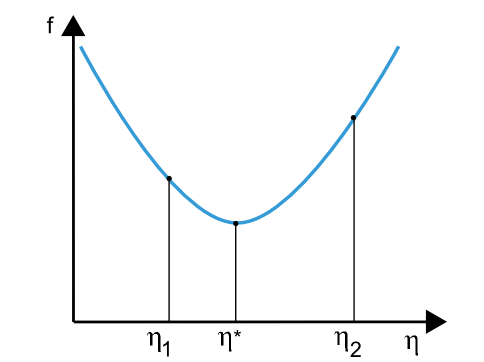
\includegraphics[height=1.65in,width=1.9in,viewport=30 0 450 360,clip]{Figures/OP_mini-1.png}
\hskip 0.1in
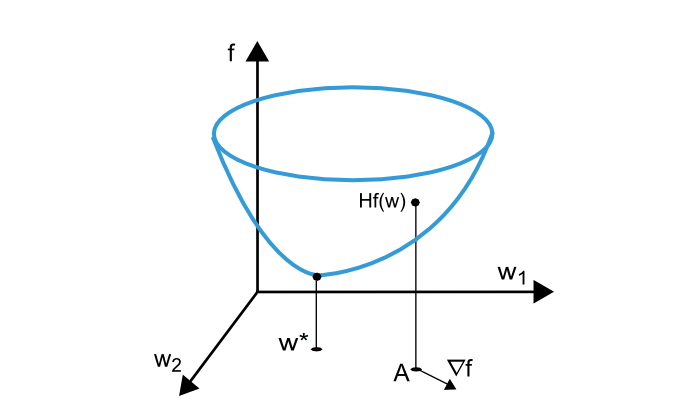
\includegraphics[height=1.65in,width=1.9in,viewport=150 20 560 390,clip]{Figures/OP_mini-2.png}
\label{OP_mini}
\end{figure}
}

\frame
{
	\frametitle{最陡下降与共轭梯度}
\begin{figure}[h!]
\centering
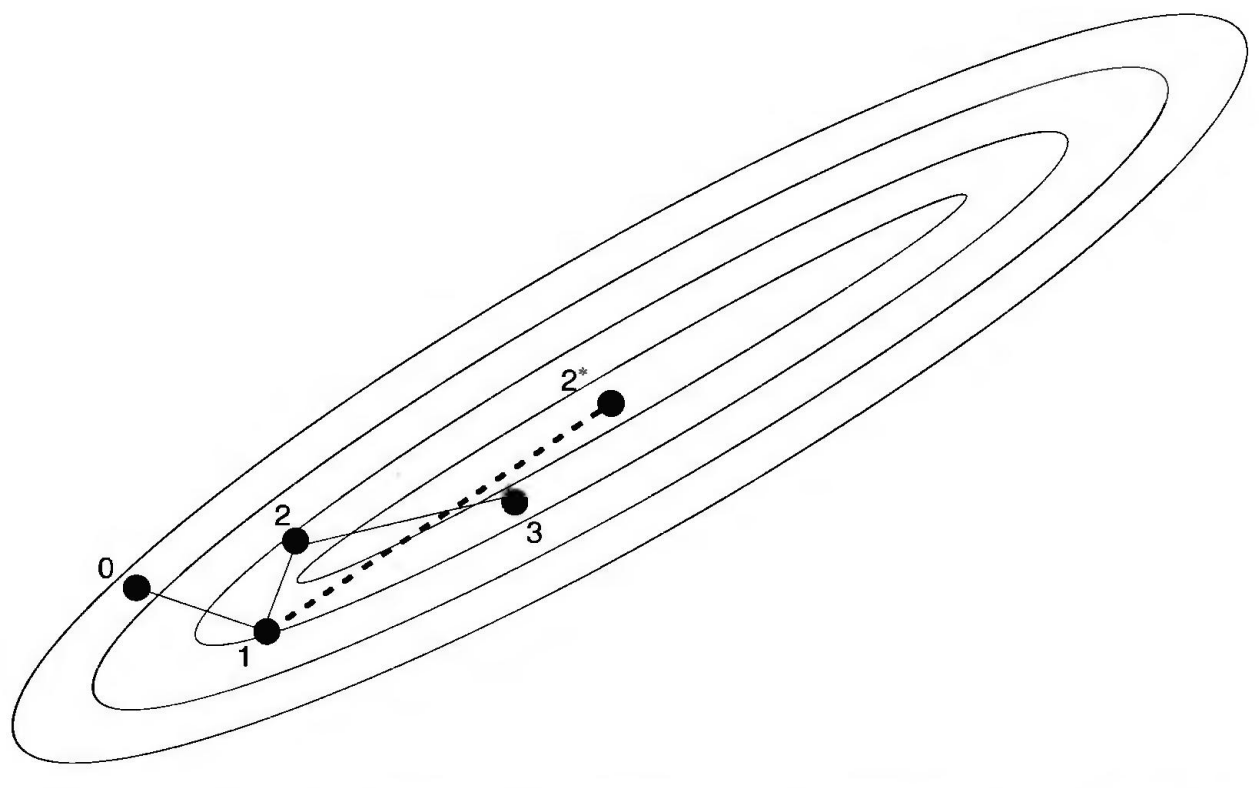
\includegraphics[height=2.0in,width=3.5in,viewport=0 0 950 590,clip]{Figures/OP_descent_CG.png}
\label{decent_CG}
\caption{\small \textrm{Schematic illustration of minimization of a function in two dimensions. The steps 1,2,3,$\cdots$ denote the steepest descent steps and the point $2^{\ast}$ denote the conjugate gradient path that reaches the exact solution after two steps if the functional is quadratic.}}%(与文献\cite{EPJB33-47_2003}图1对比)
\end{figure}
}

\subsection{电子步计算控制参数}
\frame
{
\frametitle{主要输入参数}
\begin{enumerate}
\setcounter{enumi}{3}
	\item \textcolor{red}{\textrm{Electronic Relaxation 1}}
		\begin{description}
			\item[\textcolor{blue}{ENCUT}]=200.0~eV~~\textcolor{brown}{\fontsize{7.2pt}{3.9pt}\selectfont{14.70 Ry 3.83 a.u. 3.34/3.34/3.34*2*pi/ulx,y,z}}
			\item[\textcolor{blue}{ENINI}]= 200.0~~\textcolor{brown}{\fontsize{9.2pt}{3.9pt}\selectfont{initial cutoff}}
			\item[\textcolor{blue}{ENAUG}]= 291.1 eV~~\textcolor{brown}{\fontsize{9.2pt}{3.9pt}\selectfont{ augmentation charge cutoff}}
			\item[\textcolor{blue}{NELM}]=60; \textcolor{blue}{NELMIN}=2; \textcolor{blue}{NELMDL}=0~~\textcolor{brown}{\fontsize{7.2pt}{3.9pt}\selectfont{\# of ELM stepas}} 
			\item[\textcolor{blue}{EDIFF}] = 0.1E-03 ~~\textcolor{brown}{\fontsize{9.2pt}{3.9pt}\selectfont{stopping-criterion for ELM}}
				\item[\textcolor{blue}{LREAL}]  =      F ~~\textcolor{brown}{\fontsize{9.2pt}{3.9pt}\selectfont{real-space projection}}
				\item[\textcolor{blue}{NLSPLINE}]    = F ~~\textcolor{brown}{\fontsize{9.2pt}{3.9pt}\selectfont{spline interpolate recip. space projectors}}
				\item[\textcolor{blue}{LCOMPAT}]=      F ~~\textcolor{brown}{\fontsize{9.2pt}{3.9pt}\selectfont{compatible to vasp.4.4}}
				\item[\textcolor{blue}{GGA\_COMPAT}]  = T ~~\textcolor{brown}{\fontsize{9.2pt}{3.9pt}\selectfont{GGA compatible to vasp.4.4-vasp.4.6}}
				\item[\textcolor{blue}{LMAXPAW}]     = -100 ~~\textcolor{brown}{\fontsize{9.2pt}{3.9pt}\selectfont{max onsite density}}
				\item[\textcolor{blue}{LMAXMIX}]     =    2 ~~\textcolor{brown}{\fontsize{9.2pt}{3.9pt}\selectfont{max onsite mixed and CHGCAR}}
				\item[\textcolor{blue}{VOSKOWN}]=      0 ~~\textcolor{brown}{\fontsize{9.2pt}{3.9pt}\selectfont{Vosko Wilk Nusair interpolation}}
				\item[\textcolor{blue}{ROPT}]   = 0.00000~~\textcolor{violet}{\fontsize{9.2pt}{3.9pt}\selectfont{number of grid points for non-local proj. in real space}}
		\end{description}
\end{enumerate}
   }

\frame
{
\frametitle{主要输入参数}
\begin{enumerate}
\setcounter{enumi}{4}
	\item \textcolor{red}{\textrm{Electronic Relaxation 2 (details)}}
		\begin{description}
			\item[\textcolor{red}{IALGO}]= 38~~\textcolor{brown}{\fontsize{9.2pt}{3.9pt}\selectfont{algorithm}}
			\item[\textcolor{magenta}{LDIAG}]=  T~~\textcolor{brown}{\fontsize{9.2pt}{3.9pt}\selectfont{sub-space diagonalisation (order eigenvalues)}}
			\item[\textcolor{blue}{LSUBROT}]= F~~\textcolor{brown}{\fontsize{9.2pt}{3.9pt}\selectfont{optimize rotation matrix (better conditioning)}}
			\item[\textcolor{blue}{TURBO}] = 0~~\textcolor{brown}{\fontsize{9.2pt}{3.9pt}\selectfont{\textcolor{magenta}{0=normal 1=particle mesh}}}
			\item[\textcolor{blue}{IRESTART}]= 0~~\textcolor{brown}{\fontsize{9.2pt}{3.9pt}\selectfont{\textcolor{magenta}{0=no restart 2=restart with 2 vectors}}}
			\item[\textcolor{blue}{NREBOOT}]= 0~~\textcolor{brown}{\fontsize{9.2pt}{3.9pt}\selectfont{no. of reboots}}
			\item[\textcolor{blue}{NMIN}]= 0~~\textcolor{brown}{\fontsize{9.2pt}{3.9pt}\selectfont{reboot dimension}}
			\item[\textcolor{blue}{EREF}]= 0.00~~\textcolor{brown}{\fontsize{9.2pt}{3.9pt}\selectfont{reference energy to select bands}}
			\item[\textcolor{red}{IMIX}]= 4~~\textcolor{brown}{\fontsize{9.2pt}{3.9pt}\selectfont{mixing-type and parameters}}
				\item[\textcolor{magenta}{AMIX}]= 0.40;  \textcolor{magenta}{BMIX}=  1.00\\

					\fontsize{10.2pt}{3.9pt}\selectfont{\textcolor{blue}{AMIX\_MAG} =   1.60;   \textcolor{blue}{BMIX\_MAG} =  1.00}\\
					\fontsize{10.2pt}{3.9pt}\selectfont{\textcolor{blue}{AMIN}=   0.10}\\

			\fontsize{10.2pt}{3.9pt}\selectfont{\item[\textcolor{magenta}{WC}]=100.; \textcolor{magenta}{INIMIX}=1; \textcolor{magenta}{MIXPRE}=1\\ \textcolor{blue}{MAXMIX}=-45}
		\end{description}
\end{enumerate}
   }

   \frame
   {
	   \frametitle{第一原理-分子动力学中的迭代优化:波函数}
	\begin{itemize}
		\item \textcolor{blue}{IALGO}= \textrm{2}:~\textrm{Is useful if a pre-converged WAVECAR file is read}
		\item \textcolor{blue}{IALGO}= \textrm{3}:~\textrm{Is useful if a pre-converged WAVECAR file is read}
		\item \textcolor{blue}{IALGO}= \textrm{4}:~\textrm{No optimization outside the subspace spanned by the orbitals}
		\item \textcolor{blue}{IALGO}= \textrm{5-8}:~\textrm{(Only for test)}
		\item \textcolor{blue}{IALGO}= \textrm{15-18}:~\textrm{CG} (\textrm{Should not be used any longer})
		\item \textcolor{blue}{IALGO}= \textrm{28}:~\textrm{CG} (\textrm{Mainly included for test purpose})
		\item \textcolor{blue}{IALGO}=\textcolor{red}{\textrm{38}}:~\textrm{Davidson block iteration} (\textrm{Kosugi algorithm})
			\begin{description}
				\item[\textcolor{blue}{ALGO}] = \textrm{Normal}
			\end{description}
	\end{itemize}
   }

   \frame
   {
	   \frametitle{第一原理-分子动力学中的迭代优化:波函数}
	\begin{itemize}
		\item \textcolor{blue}{IALGO}=\textrm{44}:~\textrm{Steepest descent eigenvalue minimization} \textrm{(Only for test)}
		\item \textcolor{blue}{IALGO}=\textrm{46}:~\textrm{Residuum-minimization + preconditioning} \textrm{(Only for test)}
		\item \textcolor{blue}{IALGO}=\textcolor{red}{\textrm{48}}:~\textrm{Preconditioned residuum-minimization}
			\begin{description}
				\item[\textcolor{blue}{ALGO}]=\textrm{Fast~{(RMM-DIIS)}}
			\end{description}
		\item \textcolor{blue}{IALGO}= \textrm{53}:~\textrm{damped MD with damping term automatically determinied)}
			\begin{description}
				\item[\textcolor{blue}{ALGO}]=\textrm{Damped} 
			\end{description}
		\item \textcolor{blue}{IALGO}= \textrm{54}:~\textrm{damped MD}
		\item \textcolor{blue}{IALGO}= \textrm{58}:~\textrm{Preconditioned CG}
			\begin{description}
				\item[\textcolor{blue}{ALGO}]=\textrm{All} 
			\end{description}
		\item \textcolor{blue}{IALGO}= \textcolor{red}{\textrm{90}}:~\textrm{Exact Diagonalization}
	\end{itemize}
   }

   \frame
   {
	   \frametitle{矩阵迭代对角化:~残矢与预处理}
	   \begin{itemize}
		   \item 残矢(\textrm{residual vector})
			   \begin{displaymath}
				   |R(\phi_n)\rangle=(\mathbf{H}-\varepsilon_{\mathrm{app}}\mathbf{S})|\phi_n\rangle
			   \end{displaymath}
			   由此得到近似本征态波函数的计算方法
			   \begin{displaymath}
				   \begin{aligned}
				   	|\delta\phi_n\rangle=&-\dfrac1{\mathbf{H}-\varepsilon_{\mathrm{app}}\mathbf{S}}|R(\phi_n)\rangle\\
					   |\bar\phi_n\rangle=&|\phi_n\rangle+|\delta\phi_n\rangle
				   \end{aligned}
			   \end{displaymath}
		   \item 预处理(\textrm{preconditioning}):~简化$|\delta\phi_n\rangle$求解
			   \begin{displaymath}
				   |\delta\phi_n\rangle=\mathbf{K}|R(\phi_n)\rangle
			   \end{displaymath}
			   预处理矩阵$\mathbf{K}$的计算
			   \begin{displaymath}
				   \mathbf{K}=-\sum_{\vec q}\dfrac{|\vec q\rangle\langle\vec q|}{\langle\vec q|\mathbf{H}-\varepsilon_{\mathrm{app}}\mathbf{S}|\vec q\rangle}
			   \end{displaymath}
	   \end{itemize}
   }

   \frame
   {
	   \frametitle{矩阵迭代对角化:~残矢与预处理}
	   当$\mathbf{H}$用近似$\mathbf{H}_0$可以近似表示,并且$\mathbf{H}_0$方便求解出本征态$|a_i^0\rangle$($|a_i^0\rangle$用$N_0$个平面波展开),则预处理矩阵可以进一步近似表示为:~
			   \begin{displaymath}
				   \mathbf{K}=-\sum_{i=1}^{N_0}\dfrac{|a_i^0\rangle\langle a_i^0|}{\langle a_i^0|\mathbf{H}-\varepsilon_{\mathrm{app}}\mathbf{S}|a_i^0\rangle}-\sum_{\vec q}{}^{\prime}\dfrac{|\vec q\rangle\langle\vec q|}{\langle\vec q|\mathbf{H}-\varepsilon_{\mathrm{app}}\mathbf{S}|\vec q\rangle}
			   \end{displaymath}
			   \textcolor{purple}{预处理本质上通过迭代引入更多的近似函数逼近真实函数},\textcolor{red}{不同的迭代方法预处理矩阵不同}
			   \begin{displaymath}
				   \mathbf{K}=-\sum_{\vec q}\dfrac{2|\vec q\rangle\langle\vec q|}{\frac32E^{\mathrm{kin}}(R)}\times\dfrac{27+18x+12x^2+8x^3}{27+18x+12x^2+8x^3+16x^4}
			   \end{displaymath}
			   其中$x=\dfrac{\hbar^2}{2m_e}\dfrac{q^2}{\frac32E^{\mathrm{kin}}(R)}$,$E^{\mathrm{kin}}(R)$是残矢动能
   }

   \frame
   {
	   \frametitle{\textrm{Davidson Scheme}}
	   \begin{itemize}
		   \item \textrm{Blocked Davidson}
			   \begin{displaymath}
				   \begin{aligned}
					   &\{|b_i\rangle,\cdots,i=1,2,\cdots,N_b(M+1)\}\\
					   =&\{|\phi_i^0\rangle,i=1,\cdots,N_b/|P_i^0\rangle,i=1,\cdots,N_b\\
					   &/|P_i^1\rangle,i=1,\cdots,N_b/\cdots\}
				   \end{aligned}
			   \end{displaymath}
			   这里$|P_i^0\rangle=\mathbf{K}|R(\phi_i^0\rangle)$
		   \item \textrm{Simlpe Davidson Scheme}
			   \begin{displaymath}
				   \{|b_i\rangle,\cdots,i=1,2,\cdots,2N_b\}=\{|\phi_i^0\rangle/|P_i^0\rangle,i=1,\cdots,N_b\}
			   \end{displaymath}
		   \item \textrm{Sequential band-to-band}
			   \begin{displaymath}
				   \begin{aligned}
					   |P(\phi_m)\rangle=&|p_m\rangle=\bigg(1-\sum_n|\phi_n\rangle\langle\phi_n|\mathbf{S}\bigg)\\
					   &\times\mathbf{K}(\mathbf{H}-\varepsilon_{\mathrm{app}}\mathbf{S})|\phi_m\rangle
				   \end{aligned}
			   \end{displaymath}
	   \end{itemize}
   }

   \frame
   {
	   \frametitle{\textrm{Conjugate Gradient}}
	   \begin{itemize}
		   \item 梯度矢量(\textrm{gradient vector})
			   \begin{displaymath}
				   |g(\phi_m)\rangle=|g_m\rangle=\bigg(1-\sum_m\mathbf{S}|\phi_n\rangle\langle\phi_n|\bigg)\mathbf{H}\phi_m\rangle
			   \end{displaymath}
		   \item 迭代检索方向(\textrm{search diraction})
			   \begin{displaymath}
				   |f^M\rangle=|p_m^M\rangle+\dfrac{\langle p_m^M|g_m^M\rangle}{\langle p_m^{M-1}|g_m^{M-1}\rangle}|f^{M-1}\rangle
			   \end{displaymath}
		   \item 迭代优化波函数
			   \begin{displaymath}
				   |\phi_m^{M+1}\rangle=\{|\phi_m^{M}\rangle/|f_m^M\rangle\}
			   \end{displaymath}
	   \end{itemize}
	   根据\textrm{CG}~特点,有
	   \begin{displaymath}
		   \langle p_m^M|g_m^M\rangle=\langle p_m^M|R_m^M\rangle
	   \end{displaymath}
   }

   \frame
   {
	   \frametitle{\textrm{RMM-DIIS}}
	   \begin{itemize}
		   \item \textcolor{red}{迭代正交问题}
			   \begin{displaymath}
				   \langle\phi_n|\mathbf{S}|p_m\rangle=\delta_{nm}
			   \end{displaymath}
		   \item \textcolor{blue}{优化残矢模量}:~放松正交条件
			   \begin{displaymath}
				   \begin{aligned}
					   |\phi_m^1\rangle=&|\phi_m^0\rangle+\lambda\mathbf{K}|R_m^0\rangle\\
					   |\bar\phi^M\rangle=&\sum_{i=0}^M\alpha_i|\phi_m^i\rangle\quad(M=1)\\
				   \end{aligned}
			   \end{displaymath}
			   \textcolor{purple}{当残矢可以线性表示时}
			   \begin{displaymath}
				   |\bar{R}^M\rangle=|R(\bar\phi^M)\rangle=\sum_{i=0}^M\alpha_i|R_m^i\rangle
			   \end{displaymath}
	   \end{itemize}
   }

   \frame
   {
	   \frametitle{\textrm{RMM-DIIS}}
	   \begin{itemize}
		   \item {DIIS}
			   因此要求最小化
			   \begin{displaymath}
				   \dfrac{\sum_{ij}\alpha_i^{\ast}\alpha_j\langle R_m^i|R_m^j\rangle}{\sum_{ij}\alpha_i^{\ast}\alpha_j\langle\phi_m^i|\mathbf{S}|\phi_m^j\rangle}
			   \end{displaymath}
			   上式等价于\textrm{Hermitian~}本征值问题
			   \begin{displaymath}
				   \sum_{j=0}^M\langle R_m^i|R_m^j\rangle\alpha_j=\varepsilon\sum_{j=0}^M\langle\phi_m^i|\mathbf{S}|\phi_m^j\rangle\alpha_j
			   \end{displaymath}
			   迭代过程中有
			   \begin{displaymath}
				   |\phi_m^M\rangle=|\bar\phi_m^{M-1}\rangle+\lambda\mathbf{K}|\bar{R}_m^{M-1}\rangle
			   \end{displaymath}
	   \item 残矢$|R(\phi_m^M)\rangle$直接用于扩展函数空间\\
			   参数$\lambda$须仔细选择,一般由初始计算确定
	   \end{itemize}
   }

   \frame
   {
	   \frametitle{第一原理-分子动力学中的迭代优化:~密度混合}
	\begin{itemize}
		   \item \fontsize{9.2pt}{1.9pt}{\selectfont\textrm{No mixing}}:~\textcolor{blue}{IMIX}=0\\
			   $\rho_{\mathrm{mixed}}=\rho_{\mathrm{out}}$
		   \item \fontsize{9.2pt}{1.9pt}{\selectfont\textrm{Kerker mixing}}:~\textcolor{blue}{IMIX}=1\\
			   $\rho_{\mathrm{mixed}}(\vec G)=\rho_{\mathrm{in}}(\vec G)+\textcolor{blue}{\mathrm{AMIX}}\dfrac{\vec G^2}{\vec G^2+\textcolor{blue}{\mathrm{BMIX}}^2}(\rho_{\mathrm{out}}(\vec G)-\rho_{\mathrm{in}}(\vec G))$ 
		   \item \fontsize{9.2pt}{1.9pt}{\selectfont\textrm{Damping factor($\mu$=\textcolor{blue}{AMINX})}}:~\textcolor{blue}{IMIX}=2\\
			   $\ddot{\rho}_{\mathrm{in}}(\vec G)=2\cdot\textcolor{blue}{\mathrm{AMIX}}\dfrac{\vec G^2}{\vec G^2+\textcolor{blue}{\mathrm{BMIX}}^2}(\rho_{\mathrm{out}}(\vec G)-\rho_{\mathrm{in}}(\vec G))-\mu\cdot\dot{\rho}(\vec G)$
			\begin{displaymath}
				\begin{aligned}
					\dot{\vec\rho}_{\mathrm{N+1/2}}&=\bigg((1-\mu/2)\dot{\vec\rho}_{\mathrm{N}-1/2}-2\cdot\vec F_{\mathrm{N}}\bigg)/(1+\mu/2)\\
					\vec F(\vec G)&=\textcolor{blue}{\mathrm{AMIX}}\dfrac{\vec G^2}{\vec G^2+\textcolor{blue}{\mathrm{BMIX}}^2}(\rho_{\mathrm{out}}(\vec G)-\rho_{\mathrm{in}}(\vec G))\\
					\dot{\vec\rho}_{\mathrm{N+1}}&=\dot{\vec\rho}_{\mathrm{N}}+\dot{\vec\rho}_{\mathrm{N}+1/2}
				\end{aligned}
			\end{displaymath}
		   \item \fontsize{9.2pt}{1.9pt}{\selectfont\textrm{Pulay' mixing or Broyden's method~(\textcolor{blue}{WC})}}:~\textcolor{blue}{IMIX}=4\\
	\end{itemize}
   }

   \frame
  {
	   \frametitle{第一原理-分子动力学中的迭代优化:~密度混合}
			\textcolor{blue}{WC}~(\textrm{determines Pulay's mixing or Broyden's method})
			   \begin{itemize}
				   \item $>0$:~\fontsize{9.2pt}{1.9pt}{\selectfont\textrm{Set all weights identical to \textcolor{blue}{WC}}~(\textrm{Pulay's mixing})}
				   \item $=0$:~\fontsize{9.2pt}{1.9pt}{\selectfont\textrm{Set all weight for the last step equal to 1000 and all other weights equal to 0}~(\textrm{Broyden's method})}
				   \item $<0$:~\fontsize{9.2pt}{1.9pt}{\selectfont\textrm{Try some automatic setting of the weights according to}} 
					   \begin{displaymath}
						   W_{\mathrm{iter}}=0.01\cdot|\textcolor{blue}{\mathrm{WC}}|/||\rho_{\mathrm{out}}-\rho_{\mathrm{in}}||_{\mathrm{precond}}
					   \end{displaymath}
			   \end{itemize}
		   \textcolor{blue}{INIMIX}~(\textrm{determines the initial mixing matrix, i.e. $\vec G_0$})
			\begin{itemize}
				\item 0:~\fontsize{9.2pt}{1.9pt}{\selectfont\textrm{linear mixing according to \textcolor{blue}{AMIX}}}
				\item 1:~\fontsize{9.2pt}{1.9pt}{\selectfont\textrm{Kerker mixing according to \textcolor{blue}{AMIX} and \textcolor{blue}{BMIX}}}
				\item 2:~\fontsize{9.2pt}{1.9pt}{\selectfont\textrm{no mixing (\textcolor{blue}{INIMIX}=2 and \textcolor{blue}{AMIX}=1)}}
			\end{itemize}
  }

   \frame
  {
	   \frametitle{第一原理-分子动力学中的迭代优化:~密度混合}
		 \textcolor{blue}{MIXPRE}~(\textrm{determine the metric for the Broyden's method})
				   \begin{itemize}
					   \item 0:~\fontsize{9.2pt}{1.9pt}{\selectfont\textrm{no preconditioning, metric=1}}
					   \item 1:~\fontsize{9.2pt}{1.9pt}{\selectfont\textrm{``inverse Kerker'' metric with automatically determined \textcolor{blue}{BMIX} (a range of a factor 20)}}
					   \item 2:~\fontsize{9.2pt}{1.9pt}{\selectfont\textrm{``inverse Kerker'' metric with automatically determined \textcolor{blue}{BMIX} (a range of a factor 200)}}
					   \item 3:~\fontsize{9.2pt}{1.9pt}{\selectfont\textrm{``inverse Kerker'' metric with \textcolor{blue}{BMIX}, for $\vec G>0$ $P(\vec G)=1+\dfrac{\textcolor{blue}{\mathrm{BMIX}}^2}{\vec G^2}$}}
				   \end{itemize}
  }

  \frame
  {
	  \frametitle{电荷密度混合迭代算法}
	  \begin{itemize}
		  \item 电荷密度混合迭代的核心量是电荷密度残矢$R[\rho_{\mathrm{in}}]$
			  \begin{displaymath}
				  R[\rho_{\mathrm{in}}]=\rho_{\mathrm{out}}[\rho_{\mathrm{in}}]-\rho_{\mathrm{in}}
			  \end{displaymath}
		  \item 当体系达到自洽,残矢模量为0
			  \begin{displaymath}
				  \langle R[\rho_{\mathrm{in}}]|R[\rho_{\mathrm{in}}]\rangle
			  \end{displaymath}
		  \item 简单混合:~线性混合为例
			  \begin{displaymath}
				  \rho_{\mathrm{in}}^{m+1}=\rho_{\mathrm{in}}^m+\gamma R[\rho_{\mathrm{in}}^m]
			  \end{displaymath}
		  \item \textcolor{purple}{改进简单混合:~用\textrm{Jacobian~}矩阵作为预处理改进残矢}
			  \begin{displaymath}
				  \rho_{\mathrm{in}}^{m+1}=\rho_{\mathrm{in}}^m+\mathbf{G}^1R[\rho_{\mathrm{in}}^m]
			  \end{displaymath}

	  \end{itemize}
  }

  \frame
  {
	  \frametitle{电荷密度混合迭代算法}
	  \begin{itemize}
		  \item \textrm{Kerker Scheme}
			  \begin{displaymath}
				  \mathbf{G}_q^1=A+\dfrac{\vec q^2}{\vec q^2+\vec q_0^2}
			  \end{displaymath}
		  \item \textrm{Pulay mixing}
			  \begin{itemize}
				  \item 优化电荷密度是此前若干输入电荷密度组合
					  \begin{displaymath}
						  \rho_{\mathrm{in}}^{\mathrm{opt}}=\sum_i\alpha_i\rho_{\mathrm{in}}^i
					  \end{displaymath}
				  \item \textcolor{purple}{假设残矢满足线性关系}
					  \begin{displaymath}
						  R[\rho_{\mathrm{in}}^{\mathrm{opt}}]=R[\sum_i\alpha_i\rho_{\mathrm{in}}^i]=\sum_i\alpha_iR[\rho_{\mathrm{in}}^i]
					  \end{displaymath}
					  \item 在电子数守恒约束条件$\sum\limits_i\alpha_i=1$下,优化残矢模量$\langle R[\rho_{\mathrm{in}}^{\mathrm{opt}}]|R[\rho_{\mathrm{in}}^{\mathrm{opt}}]\rangle$
			  \end{itemize}
	  \end{itemize}
  }

  \frame
  {
	  \frametitle{电荷密度混合迭代算法:\textrm{Pulay mixing}}
	  \begin{itemize}
		  \item 优化系数$\alpha_i$:
			  \begin{displaymath}
				  \alpha_i=\dfrac{\sum_jA_{ji}^{-1}}{\sum_{kj}A_{kj}^{-1}}\quad A_{ij}=\langle R[\rho_{\mathrm{in}}^j]|R[\rho_{\mathrm{in}}^i]\rangle
			  \end{displaymath}
		  \item 迭代中的优化输入电荷密度
			  \begin{displaymath}
				  \rho_{\mathrm{in}}^{\mathrm{opt}}=\rho^m+\sum_{i=1}^{m-1}\bar\alpha_i\Delta\rho^i
			  \end{displaymath}
			  这里$\rho^m=\rho_{\mathrm{in}}^m$;~$\Delta\rho^i=\rho_{\mathrm{in}}^{i+1}-\rho_{\mathrm{in}}^{i}$;$R^m=R[\rho_{\mathrm{in}}^m]$
			  $\bar\alpha_i=-\sum\limits_{j=1}^{m-1}\bar{A}_{ji}^{-1}\langle\Delta R^j|R^m\rangle$;~$\bar{A}_{ji}=\langle\Delta R^j|\Delta R^i\rangle$;\\$\Delta R^i=R[\rho_{\mathrm{in}}^{i+1}]-R[\rho_{\mathrm{in}}^{i}]$

	  \end{itemize}
  }

  \frame
  {
	  \frametitle{电荷密度混合迭代算法:\textrm{Pulay mixing}}
	  \begin{itemize}
		  \item \textrm{Pulay mixing}
			  \begin{displaymath}
				  \begin{aligned}
					  \rho_{\mathrm{in}}^{m+1}=&\rho_{\mathrm{in}}^{\mathrm{opt}}+\mathbf{G}^1R[\rho_{\mathrm{in}}^{\mathrm{opt}}]\\
					  =&\rho_{\mathrm{in}}^{m}++\mathbf{G}^1R^m+\sum_{i=1}^{m-1}\bar\alpha_i(\Delta\rho^i+\mathbf{G}^1\Delta R^i)
				  \end{aligned}
			  \end{displaymath}
			  式中$\mathbf{G}^1$是常数,一般选择为\textrm{Kerker~}的结果
	  \end{itemize}
  }

  \frame
  {
	  \frametitle{电荷密度混合迭代算法:\textrm{Broyden mixing}}
	  \begin{itemize}
		  \item \textrm{quasi-Newton method}
			  \begin{displaymath}
				  R[\rho]=R[\rho_{\mathrm{in}}^{m}]-\mathbf{J}^m(\rho-\rho_{\mathrm{in}}^{m})
			  \end{displaymath}
		  \item 因为要求$R[\rho^{\ast}]$为0
			  \begin{displaymath}
				  \rho^{\ast}=\rho_{\mathrm{in}}^{m}-(\mathbf{J}^m)^{-1}R[\rho_{\mathrm{in}}^{m}]
			  \end{displaymath}
		  \item 实际计算中
			  \begin{displaymath}
				  \rho_{\mathrm{in}}^{m+1}=\rho_{\mathrm{in}}^{m}-(\mathbf{J}^m)^{-1}R[\rho_{\mathrm{in}}^{m}]
			  \end{displaymath}
		  \item 这一类算法的区别:~迭代过程中矩阵$\mathbf{J}^m$选择方式不同(以下取$\mathbf{G}^m=(\mathbf{J}^m)^{-1}$)\\
			  改进的\textrm{Broyden~}方法推导:~通过误差函数的最小二乘解
			  \begin{displaymath}
				  E=w_0||\mathbf{G}^{m+1}-\mathbf{G}^m||^2+\sum_{i=1}^m w_i||\Delta\rho^i+\mathbf{G}^{m+1}\Delta R^i||^2
			  \end{displaymath}
			  计算$\mathbf{G}^m$
	  \end{itemize}
  }

  \frame
  {
	  \frametitle{电荷密度混合迭代算法:\textrm{Broyden mixing}}
	  \begin{itemize}
		  \item $\mathbf{G}^m$的计算
			  \begin{displaymath}
				  \mathbf{G}^{m+1}=\mathbf{G}^1-\sum_{k=1}^m|Z_k^m\rangle\langle\Delta R^k\rangle
			  \end{displaymath}
			  这里
			  \begin{displaymath}
				  \begin{aligned}
					  |Z_k^m\rangle=&\sum_{n=1}^m\beta_{kn}w_kw_n|u^n\rangle+\sum_{n=1}^{m-1}\bar\beta_{kn}|Z_n^{m-1}\rangle\\
					  |u^n\rangle=&\mathbf{G}^1|\Delta R^n\rangle+|\Delta\rho^n\rangle
					  \beta_{kn}=&\big(w_0^2+\bar{A}\big)_{kn}^{-1}\quad \bar{A}_{kn}=w_kw_n\langle\Delta R^n|\Delta R^k\rangle\\
					  \bar\beta_{kn}=&\delta_{kn}-\sum_{j=1}^mw_kw_j\beta_{kj}\langle\Delta R^n|\Delta R^j\rangle
				  \end{aligned}
			  \end{displaymath}
	  \end{itemize}
	  可以近似地取$\bar\beta_{kn}=w_0^2\beta_{kn}$
   }

  \frame
  {
	  \frametitle{\textrm{Pulay mixing}与\textrm{Broyden mixing}}
	  \begin{itemize}
		  \item \textrm{Pulay mixing}:
			  \begin{displaymath}
				  w_0\rightarrow0\quad w_0<<w_n
			  \end{displaymath}
			  令$w_n=1$,可有\textrm{Pulay mixing}的$\mathbf G^m$迭代
			  \begin{displaymath}
				  \mathbf{G}^m=\mathbf{G}^1-\sum_{k,n=1}^{m-1}\beta_{kn}|u^n\rangle\langle\Delta R^k|
			  \end{displaymath}
		  \item \textrm{Broyden mixing}:
			  \begin{displaymath}
				  w_i=0~(i<m)\quad w_0<<w_m
			  \end{displaymath}
			  \textrm{Broyden mixing}的迭代可简化为
			  \begin{displaymath}
				  \begin{aligned}
					  |Z_k^m\rangle=&|Z_k^{m-1}\rangle\quad k<m\\
					  |Z_m^m\rangle=&\dfrac1{||\Delta R^m||}\bigg(|u^m\rangle-\sum_{k=1}^{m-1}\langle\Delta R^k|\Delta R^m\rangle|Z_k^{m-1}\rangle\bigg)
				  \end{aligned}
			  \end{displaymath}
	  \end{itemize}
  }

  \frame
  {
	  \frametitle{\textrm{Preconditioning}与\textrm{metric}}
	  \begin{itemize}
		  \item 初始矩阵$\mathbf{G}^1$\\
			  为简便起见,$\mathbf{G}^1$取为\textrm{Kerker~}矩阵$G^1=A\dfrac{q^2}{q^2+q_0^2}$
	  		\\\textcolor{magenta}{对于\textrm{Pulay's method},推荐}:~
			$A=0.8$,$q_0=1.5\mbox{\textrm{\AA}}^{-1}$
		  \item 优化标度(\textrm{optimized metric}):~\textcolor{blue}{尽可能少的迭代次数}\\
			  对标量积,引入权重因子$f_q$
			  \begin{displaymath}
				  \langle A|B\rangle=\sum_qf_qA_q\cdot B_q\quad f_q=\dfrac{q^2+q_1^2}{q^2}
			  \end{displaymath}
			  \textcolor{blue}{经验表明,对于复杂金属体系,可以很好提升优化标度}
		  \item 对于倒空间,对波矢$q$很大的波函数,可以不考虑混合
			  \begin{displaymath}
				  \rho_{\mathrm{in}}^{m+1}=\rho_{\mathrm{out}}^{m}
			  \end{displaymath}
	  \end{itemize}
  }

\subsection{物性计算控制参数}
\frame
{
\frametitle{主要输入参数}
\textcolor{red}{主要原子参数}
\begin{itemize}
	\item \textcolor{blue}{POMASS} =  26.98~~\textcolor{brown}{\fontsize{9.2pt}{3.9pt}\selectfont{Mass of Ions in am}}\\

	\item \textcolor{blue}{ZVAL}   =   3.00~~\textcolor{brown}{\fontsize{9.2pt}{3.9pt}\selectfont{Ionic Valenz}}\\

	\item \textcolor{blue}{RWIGS}  =  -1.00~~\textcolor{brown}{\fontsize{9.2pt}{3.9pt}\selectfont{Atomic Wigner-Seitz radii}}\\
		
	\item \textcolor{blue}{VCA}    =   1.00~~\textcolor{brown}{\fontsize{9.2pt}{3.9pt}\selectfont{virtual crystal weights}}\\
   
	\item \textcolor{blue}{NELECT} =       3.0000 ~~\textcolor{brown}{\fontsize{9.2pt}{3.9pt}\selectfont{total number of electrons}}\\

	\item \textcolor{blue}{NUPDOWN}=      -1.0000 ~~\textcolor{brown}{\fontsize{9.2pt}{3.9pt}\selectfont{fix difference up-down}}
\end{itemize}

\begin{enumerate}
\setcounter{enumi}{5}
\item \textcolor{red}{\textrm{DOS related values:}}
	\begin{description}
		\item[\textcolor{blue}{EMIN}]=  10.00;   \textcolor{blue}{EMAX}   =-10.00~~\textcolor{brown}{\fontsize{9.2pt}{3.9pt}\selectfont{energy-range for DOS}}
		\item[\textcolor{blue}{EFERMI}] =   0.00
		\item[\textcolor{magenta}{ISMEAR}] =    -5;   \textcolor{magenta}{SIGMA}  =   0.20~~\textcolor{blue}{\fontsize{9.2pt}{3.9pt}\selectfont{broadening in eV\\\textcolor{magenta}{-4-tet -1-fermi 0-gaus}}}
	\end{description}
\end{enumerate}
   }

\frame
{
	\frametitle{各种$\vec k$~空间积分方法的比较}
\vskip -7pt
\begin{footnotesize}
\arrayrulewidth=0.4pt
\doublerulesep=0.4pt
\begin{table}[!h]
\tabcolsep 0pt \vspace*{-12pt}
%\begin{minipage}{\textwidth}
\label{tab:magno-1}
\centering
\def\temptablewidth{1.01\textwidth}
{\rule{\temptablewidth}{0.8pt}}
\begin{tabular*} {\temptablewidth}{|c@{\extracolsep{\fill}}|c|c|c|c|}
	\multirow{3}{*}{\textcolor{red}{积分方案}}	&\multicolumn{4}{c|}{\textcolor{blue}{布点方案}:~\textrm{Monkhorst-Pack}~方法} \\\cline{2-5}
	&\multirow{2}{*}{\textrm{Fermi-Dirac}~方法} &\multicolumn{2}{c|}{\textrm{Methfessel-Paxton}~方法} &\multirow{2}{*}{\textrm{Tetrahedron}~方法}\\\cline{3-4}
& &\textrm{Gaussian~} &$N>0$ & \\ \hline
半导体、&\multirow{2}{*}{\textcolor{blue}{$\texttimes$}} &$\delta\leqslant0.05$ &\multirow{2}{*}{\textcolor{red}{$\texttimes$}} &\textcolor{blue}{\textrm{DOS \& total-Energy}}\\
绝缘体 & &\textcolor{blue}{$\checkmark$} & &\textcolor{red}{$\checkmark$} \\\hline
导体、 & \multirow{2}{*}{\textcolor{blue}{$\checkmark$}} & \multicolumn{2}{c|}{\textcolor{blue}{\textrm{Phonon \& relaxation}}} &\textcolor{blue}{\textrm{DOS \& total-Energy}} \\
金属 & &\multicolumn{2}{c|}{\textcolor{red}{$\checkmark$}}  &\textcolor{red}{$\checkmark$} \\\hline
\multirow{2}{*}{\textrm{supercell}} &\multirow{2}{*}{\textcolor{blue}{$\checkmark$}} &\multicolumn{2}{c|}{\multirow{2}{*}{\textcolor{red}{$\checkmark$}}} &\multirow{2}{*}{\textcolor{red}{$\texttimes$}}\\
& &\multicolumn{2}{c|}{} &\\
\end{tabular*}
{\rule{\temptablewidth}{1pt}}\\
%\end{center}1
%\end{minipage}
\end{table}
\end{footnotesize}
}

\frame
{
\frametitle{主要输入参数}
\begin{enumerate}
\setcounter{enumi}{6}
 \item \textcolor{red}{\textrm{Intra band minimization:}}
	 \begin{description}
		 \item[\textcolor{blue}{WEIMIN}] = 0.0000     ~~\textcolor{brown}{\fontsize{9.2pt}{3.9pt}\selectfont{energy-eigenvalue tresh-hold}}
		 \item[\textcolor{blue}{EBREAK}] =  0.50E-05  ~~\textcolor{brown}{\fontsize{9.2pt}{3.9pt}\selectfont{absolut break condition}}
		 \item[\textcolor{blue}{DEPER}]  =   0.30     ~~\textcolor{brown}{\fontsize{9.2pt}{3.9pt}\selectfont{relativ break condition}}

		 \item[\textcolor{blue}{TIME}]   =   0.40     ~~\textcolor{brown}{\fontsize{9.2pt}{3.9pt}\selectfont{timestep for ELM}}
	 \end{description}
	 \begin{description}
		 \fontsize{9.2pt}{3.9pt}\selectfont{\item[\textcolor{blue}{volume/ion in A,a.u.}] = 17.23~~116.28
		 \item[\textcolor{blue}{Fermi-wavevector in a.u.,A,eV,Ry}] = 0.914151~1.727495~11.370015~0.835673
		 \item[\textcolor{blue}{Thomas-Fermi vector in A}] = 2.038745}
	 \end{description}
 \item \textcolor{red}{\textrm{Write flags}}
	 \begin{description}
		 \item[\textcolor{blue}{LWAVE}]  = T ~~\textcolor{brown}{\fontsize{9.2pt}{3.9pt}\selectfont{write WAVECAR}}
		 \item[\textcolor{blue}{LCHARG}] = T ~~\textcolor{brown}{\fontsize{9.2pt}{3.9pt}\selectfont{write CHGCAR}}
		 \item[\textcolor{blue}{LVTOT}]  = T ~~\textcolor{brown}{\fontsize{9.2pt}{3.9pt}\selectfont{write LOCPOT, total local potential}}
		 \item[\textcolor{blue}{LVHAR}]  = F ~~\textcolor{brown}{\fontsize{9.2pt}{3.9pt}\selectfont{write LOCPOT, Hartree potential only}}
		 \item[\textcolor{blue}{LELF}]   = F ~~\textcolor{brown}{\fontsize{9.2pt}{3.9pt}\selectfont{write electronic localiz. function (ELF)}}
		 \item[\textcolor{blue}{LORBIT}] = 0 ~~\textcolor{magenta}{\fontsize{9.2pt}{3.9pt}\selectfont{0 simple, 1 ext, 2 COOP (PROOUT)}}
	 \end{description}
\end{enumerate}
   }


\frame
{
\frametitle{主要输入参数}
\begin{enumerate}
\setcounter{enumi}{8}
  \item \textcolor{red}{\textrm{Dipole corrections}}
	  \begin{description}
		  \item[\textcolor{blue}{LMONO}] = F ~~\textcolor{brown}{\fontsize{9.2pt}{3.9pt}\selectfont{monopole corrections only (constant potential shift)}}
		  \item[\textcolor{blue}{LDIPOL}] = F ~~\textcolor{brown}{\fontsize{9.2pt}{3.9pt}\selectfont{correct potential (dipole corrections)}}
		  \item[\textcolor{blue}{IDIPOL}] = 0 ~~\textcolor{brown}{\fontsize{9.2pt}{3.9pt}\selectfont{\textcolor{magenta}{1-x, 2-y, 3-z, 4-all directions}}}
		  \item[\textcolor{blue}{EPSILON}]= 1.0000000 ~~\textcolor{brown}{\fontsize{9.2pt}{3.9pt}\selectfont{bulk dielectric constant}}
	  \end{description}

  \item \textcolor{red}{\textrm{Exchange correlation treatment:}}
	  \begin{description}
		  \item[\textcolor{blue}{GGA}] = -- ~~\textcolor{brown}{\fontsize{9.2pt}{3.9pt}\selectfont{GGA type}}
		  \item[\textcolor{blue}{LEXCH}] = 8 ~~\textcolor{brown}{\fontsize{9.2pt}{3.9pt}\selectfont{internal setting for exchange type}}
		  \item[\textcolor{blue}{VOSKOWN}] = 0 ~~\textcolor{brown}{\fontsize{9.2pt}{3.9pt}\selectfont{Vosko Wilk Nusair interpolation}}
		  \item[\textcolor{blue}{LHFCALC}] = F ~~\textcolor{brown}{\fontsize{9.2pt}{3.9pt}\selectfont{Hartree Fock is set to}}
		  \item[\textcolor{blue}{LHFONE}] = F ~~\textcolor{brown}{\fontsize{9.2pt}{3.9pt}\selectfont{Hartree Fock one center treatment}}
		  \item[\textcolor{blue}{AEXX}] = 0.0000 ~~\textcolor{brown}{\fontsize{9.2pt}{3.9pt}\selectfont{exact exchange contribution}}
	  \end{description}
\end{enumerate}
   }

\frame
{
\frametitle{主要输入参数}
\begin{enumerate}
\setcounter{enumi}{10}
 \item \textcolor{red}{\textrm{Linear response parameters}}
	  \begin{description}
		  \item[\textcolor{blue}{LEPSILON}]= F ~~\textcolor{brown}{\fontsize{9.2pt}{3.9pt}\selectfont{determine dielectric tensor}}
		  \item[\textcolor{blue}{LRPA}] = F ~~\textcolor{brown}{\fontsize{9.2pt}{3.9pt}\selectfont{only Hartree local field effects (RPA)}}
		  \item[\textcolor{blue}{LNABLA}] = F ~~\textcolor{brown}{\fontsize{9.2pt}{3.9pt}\selectfont{use nabla operator in PAW spheres}}
		  \item[\textcolor{blue}{LVEL}] = F ~~\textcolor{brown}{\fontsize{9.2pt}{3.9pt}\selectfont{velocity operator in full k-point grid}}
		  \item[\textcolor{blue}{LINTERFAST}] = F ~~\textcolor{brown}{\fontsize{9.2pt}{3.9pt}\selectfont{fast interpolation}}
		  \item[\textcolor{blue}{KINTER}] = 0 ~~\textcolor{brown}{\fontsize{9.2pt}{3.9pt}\selectfont{interpolate to denser k-point grid}}
		  \item[\textcolor{blue}{CSHIFT}] = 0.1000 ~~\textcolor{brown}{\fontsize{9.2pt}{3.9pt}\selectfont{complex shift for real part using Kramers-Kr\"onig relation}}
		  \item[\textcolor{blue}{OMEGAMAX}]=  -1.0 ~~\textcolor{brown}{\fontsize{9.2pt}{3.9pt}\selectfont{maximum frequency}}
		  \item[\textcolor{blue}{DEG\_THRESHOLD}] = 0.2000000E-02 ~~\textcolor{brown}{\fontsize{9.2pt}{3.9pt}\selectfont{threshold for treating states as degnerate}}
		  \item[\textcolor{blue}{RTIME}] = 0.100 ~~\textcolor{brown}{\fontsize{9.2pt}{3.9pt}\selectfont{relaxation time in fs}}
	  \end{description}
\end{enumerate}
   }

\frame
{
\frametitle{主要输入参数}
\begin{enumerate}
\setcounter{enumi}{11}
 \item \textcolor{red}{\textrm{Orbital magnetization related:}}
	  \begin{description}
		  \item[\textcolor{blue}{ORBITALMAG}]= F ~\textcolor{brown}{\fontsize{9.2pt}{3.9pt}\selectfont{switch on orbital magnetization}}
		  \item[\textcolor{blue}{LCHIMAG}]   = F ~\textcolor{brown}{\fontsize{9.2pt}{3.9pt}\selectfont{perturbation theory with respect to B field}}
		  \item[\textcolor{blue}{DQ}] = 0.00100 ~\textcolor{brown}{\fontsize{8.2pt}{3.9pt}\selectfont{ dq finite difference perturbation B field}}
	  \end{description}
\end{enumerate}
   }

   \appendix
   \section{附录1:~函数优化与矩阵对角化}
   \subsection{函数优化的基本方法}
\frame
{
	\frametitle{\textrm{Method of steepest descent}}
	对于函数$f(\mathbf{x}_0)$当前位置$\mathbf{x}_0$的负梯度方向$\mathbf{g}_0$满足
	\begin{displaymath}
		\mathbf{g}_0=-\nabla f(\mathbf{x}_0)
	\end{displaymath}
	用$\mathbf{g}_0$方向作为搜索方向,
	\begin{displaymath}
		\mathbf{x}=\mathbf{x}_0+\lambda\mathbf{g}_0,\qquad \lambda>0
	\end{displaymath}
	因为负的梯度方向为当前位置的最快下降方向,所以被称为“\textcolor{blue}{最陡下降法}”\\
	对函数$f$最小化参数$\lambda$,可确定下一步$\mathbf{x}_1$,可有
	\begin{displaymath}
		\dfrac{\mathrm{d}}{\mathrm{d}\lambda}f(\mathbf{x}_0+\lambda\mathbf{g})_0=\mathbf{g}_0\cdot\nabla f(\mathbf{x}_1)=\mathbf{g}_0\cdot\mathbf{g}_1=0
	\end{displaymath}
	因此\textcolor{red}{最速下降法最近邻两步的梯度彼此相互垂直}\\
	\textcolor{purple}{最陡下降法的收敛:~}\\靠近极小值时收敛速度减慢,越接近目标,步长越小,前进越慢
}

\frame
{
	\frametitle{\textrm{Conjugate gradient}}
	\fontsize{9.2pt}{3.9pt}\selectfont{假设函数在接近极值附件,近似有二次函数的形式
	\begin{displaymath}
		f(\mathbf{x})=f_0+\frac12\mathbf{x}\cdot\mathbf{H}{\mathbf{x}}+\cdots
	\end{displaymath}
	其中$\mathbf{H}$是\textcolor{blue}{\textrm{Hessian}矩阵},定义为
	\begin{displaymath}
		H_{ij}=\dfrac{\partial^2f(\mathbf{x})}{\partial x_i\partial x_j}
	\end{displaymath}
	当$f$的偏导连续,则$\mathbf{H}$是对称矩阵,并且一般要求$\mathbf{H}$是正定的
	\vskip 20pt
	设从点$\mathbf{x}_i$出发沿方向$\mathbf{h}_i$(\textcolor{blue}{不再限于梯度$\mathbf{g}_i$方向}),前进到点$\mathbf{x}_{i+1}$,由根据最小化要求
	\begin{displaymath}
		\mathbf{h}_i\cdot\nabla f(\mathbf{x}_{i+1})=0
	\end{displaymath}
	为确定$\mathbf{x_{i+1}}$点的继续前进方向$\mathbf{h}_{i+1}$,设$\mathbf{x}_{i+1}$可由$\mathbf{x}_i+\lambda\mathbf{h}_{i+1}$得到,因此$\mathbf{x}_{i+1}$的梯度
	\begin{displaymath}
		\mathbf{g}_{i+1}=\nabla f(\mathbf{x}_{i+1})=-\mathbf{H}\mathbf{x}_{i+1}=-\mathbf{H}(\mathbf{x}_{i}+\lambda\mathbf{h}_{i+1})
	\end{displaymath}}
}

\frame
{
	\frametitle{\textrm{Conjugate gradient}}
	与方向$\mathbf{h}_i$相比,梯度的改变为
	\begin{displaymath}
		\Delta\mathbf{g}=-\lambda\mathbf{H}\mathbf{h}_{i+1}
	\end{displaymath}

	根据最小化要求,梯度的改变与$\mathbf{h}_i$方向正交
	\begin{displaymath}
		\mathbf{h}_i\cdot\mathbf{H}\mathbf{h}_{i+1}=0
	\end{displaymath}
	共轭梯度法算法:对于给定函数
	\begin{itemize}
		\item 已知初值$\mathbf{x}_0$和梯度$\mathbf{g}_0$,取初始方向$\mathbf{h_0}=\mathbf{g}_0$(\textcolor{blue}{最陡下降})
		\item 根据递推关系确定
			\begin{displaymath}
				\begin{aligned}
					\mathbf{g}_{i_+1}=&\mathbf{g}_{i_+1}-\lambda_i\mathbf{H}\mathbf{h}_{i}\qquad \lambda_i=\dfrac{\mathbf{g}_i\cdot\mathbf{g}_i}{\mathbf{g}_i\cdot\mathbf{H}\mathbf{h}_i}\\	
					\mathbf{h}_{i_+1}=&\mathbf{g}_{i_+1}+\gamma_i\mathbf{h}_{i}\qquad \gamma_i=-\dfrac{\mathbf{g}_{i+1}\cdot\mathbf{H}\mathbf{h}_i}{\mathbf{h}_i\cdot\mathbf{H}\mathbf{h}_i}\\	
					\mathbf{x}_{i_+1}=&\mathbf{x}_{i}+\lambda_i\mathbf{h}_{i}
				\end{aligned}
			\end{displaymath}
	\end{itemize}
	\textcolor{purple}{共轭梯度法:~步收敛性,稳定性高,不需要任何外来参数}
}

\frame
{
	\frametitle{\textrm{Quasi-Newton Methods}}
	\fontsize{9.2pt}{3.9pt}\selectfont{求解方程
	\begin{displaymath}
		f(\mathbf{x})=\mathbf{x}
	\end{displaymath}
	$\mathbf{x}$是函数$f(\mathbf{x})$的\textcolor{red}{不动点}
	
	对这类问题的求解,可以利用迭代关系
	\begin{displaymath}
		\mathbf{x}_{i+1}=f(\mathbf{x}_i)\qquad (i=1,2,3,\cdots)
	\end{displaymath}
	这称为\textcolor{blue}{不动点迭代法}

	另一种求解策略是定义残量
	\begin{displaymath}
		R[\mathbf{x}]=f(\mathbf{x})-\mathbf{x}
	\end{displaymath}
	最小化残量的模$|R[\mathbf{x}]|$,特别是当残量$R[\mathbf{x}]$近似是$\mathbf{x}$的线性函数,可有\textcolor{purple}{Jacobian}矩阵
	\begin{displaymath}
		\mathbf{J}=\dfrac{\delta R[\mathbf{x}]}{\delta\mathbf{x}}
	\end{displaymath}
	可通过迭代关系求解原方程的解
	\begin{displaymath}
		\mathbf{x}_{i+1}=\mathbf{x}_{i}-\mathbf{J}^{-1}R[\mathbf{x}_{i}]
	\end{displaymath}}
}

\subsection{相似矩阵与直接对角化}
\frame
{
	\frametitle{相似矩阵}
\textcolor{blue}{相似矩阵}:~设$\mathbf{A}$,$\mathbf{B}$都是\textrm{n}阶矩阵,若有可逆矩阵$\mathbf{P}$,使得
	\begin{displaymath}
		\mathbf{P}^{-1}\mathbf{A}\mathbf{P}=\mathbf{B}
	\end{displaymath}
	则称$\mathbf{B}$是$\mathbf{A}$的相似矩阵,或说$\mathbf{A}$和$\mathbf{B}$相似
	\begin{itemize}
		\item 相似矩阵具有\textcolor{red}{相同的}\textcolor{blue}{本征向量}和\textcolor{blue}{本征值}
		\item 若$\mathbf{A}$相似于\textcolor{brown}{对角矩阵}$\boldsymbol{\Lambda}$,则$\boldsymbol{\Lambda}$主对线上元素是$\mathbf{A}$的\textrm{n}个本征值
		\item \textrm{n}阶方阵$\mathbf{A}$能与对角矩阵$\boldsymbol{\Lambda}$相似的充分必要条件:~$\mathbf{A}$有\textrm{n}个\textcolor{magenta}{线性无关}的本征向量
		\item 实对称矩阵的特征值为实数
		\item \textcolor{purple}{实对称矩阵不同的本征值所对应的本征向量线性无关}
	\end{itemize}
}

\frame
{
	\frametitle{\textrm{QR}分解与矩阵的对角化}
	\fontsize{9.2pt}{3.9pt}\selectfont{\textrm{QR~}方法本质上是一种变换方法,是计算一般矩阵(中小型矩阵)的全部本征值的最有效方法之一
\vskip 5pt
	所谓\textrm{QR}分解,就是将一个矩阵(以实对称方针为例)分解成一个\textcolor{blue}{正交矩阵}和一个\textcolor{blue}{上三角矩阵}。即
	\begin{displaymath}
		\mathbf{A}=\mathbf{Q}\mathbf{R}
	\end{displaymath}
	其中$\mathbf{Q}$是正交矩阵,即$\mathbf{Q}$中的列向量互相正交,即
	\begin{displaymath}
		\mathbf{Q}^{-1}\mathbf{Q}=\mathbf{I} 
	\end{displaymath}
	$\mathbf{R}$是上三角矩阵,可得到新矩阵$\mathbf{B}$
	\begin{displaymath}
		\mathbf{B}=\mathbf{R}\mathbf{Q}=\mathbf{Q}^{-1}\mathbf{A}\mathbf{Q}
	\end{displaymath}
	$\mathbf{B}$与$\mathbf{A}$是相似矩阵,可以再对$\mathbf{B}$进行\textrm{QR~}分解\\
	\textcolor{red}{当$\mathbf{A}$为非奇异矩阵时,这个分解是唯一的}
	\begin{itemize}
		\item 实现\textrm{QR}分解的算法有多种,包括\textrm{Gram–Schmidt~}正交化,\textrm{Householder~}变换,以及\textrm{Givens~}旋转等
	\end{itemize}}
}

\subsection{稀疏矩阵的迭代对角化基本算法}
\frame
{
	\frametitle{矩阵的迭代对角化}
	\begin{itemize}
		\item 矩阵的直接对角化计算量 $O(N^3)$
		\item 矩阵的迭代对角化 $O(N_0^2\times N\ln N)\quad N_0\ll N$
	\end{itemize}
	\textcolor{blue}{迭代求本征值的思想是\textrm{Jacobian~}于\textrm{1846~}年提出的}\upcite{Crelle30-51_1846}\\
	其基本思想是
	\begin{displaymath}
		(H-\varepsilon^n)|\psi^n\rangle=|R[\psi^n]\rangle
	\end{displaymath}
	这里$n$是迭代步数,$|\psi^n\rangle$和$\varepsilon^n$分别是本征态和本征值,$|R[\psi^n]\rangle$是残矢量
	\vskip 10pt
	在电子态计算过程中,选择适当的基函数,可以使\textrm{Schr\"odinger~}方程的矩阵接近对角阵,因此可有
	\begin{displaymath}
		|\psi\rangle=\mathbf{D}^{-1}(\mathbf{H}-\varepsilon)|\psi\rangle+|\psi\rangle
	\end{displaymath}
	这里$\mathbf{D}$是非奇异矩阵,与$\mathbf{H}$矩阵有关,可根据需要选取多种形式
}

\frame
{
	\frametitle{稀疏矩阵的\textrm{Lanczos~}算法}
	对于稀疏矩阵$\mathbf{A}$,取任意矢量$\psi_0$(要求归一),构造矢量$\psi_1$(同样要求归一,并与$\psi_0$正交),满足
	\begin{displaymath}
		\mathbf{A}\psi_0=a_0\psi_0+b_0\psi_1
	\end{displaymath}
	由此确定$a_0$、$b_0$、$\psi_1$
	\begin{displaymath}
		\begin{aligned}
			a_0&=\langle\psi_0|\mathbf{A}|\psi_0\rangle\\
			b_0\psi_1&=\mathbf{A}\psi_0-a_0\psi_0\\
			||\psi_1||&=1
		\end{aligned}
	\end{displaymath}
	进而可构造$\psi_2$:
	\begin{displaymath}
		\mathbf{A}\psi_1=c_1\psi_0+a_1\psi_1+b_1\psi_2
	\end{displaymath}
	要求$\psi_2$与$\psi_0$、$\psi_1$正交归一条件,确定$\psi_2$,$a_1$,$b_1$,$c_1$
}

\frame
{
	\frametitle{稀疏矩阵的\textrm{Lanczos~}算法}
	根据递推关系有
	\begin{displaymath}
		\mathbf{A}\psi_p=\sum_{q=0}^{p-1}c_p^{(q)}\psi_q+a_q\psi_p+b_p\psi_{p+1}
	\end{displaymath}
	这里$\psi_{p+1}$将与所有之前的$\psi_q$(\textrm{processors})正交

	利用矩阵$\mathrm{A}$的\textrm{Hermitian},因此可有等式
	\begin{displaymath}
		c_p^{(q)}=\langle\psi_q|\mathbf{A}\psi_p\rangle=\langle\mathbf{A}\psi_q|\psi_p\rangle=0
	\end{displaymath}
	即矢量$\psi_p$垂直于矢量$\mathbf{A}\psi_q$,由此可得
	\begin{displaymath}
		c_p^{(p-1)}=\langle\psi_{p-1}|\mathbf{A}\psi_p\rangle=\langle\mathbf{A}\psi_{p-1}|\psi_p\rangle=b_{p-1}
	\end{displaymath}
	经过$p$步迭代后
	\begin{displaymath}
		\mathbf{A}\psi_p=b_{p-1}\psi_{p-1}+a_p\psi_p+b_p\psi_{p+1}
	\end{displaymath}
	这里$\psi_{p+1}$要求与$\psi_p$和$\psi_{p-1}$满足正交归一条件
}

\subsection{密度混合与迭代算法}
\frame
{
	\frametitle{\textrm{Pulay DIIS full-subspace Method}}
	\textrm{DIIS(Direct inversion in the iterative subspace)}的基本思想:~\\
	\textcolor{blue}{迭代中,将此前每一步迭代得到的$\mathbf{x}_i$组合,实现当前残量最小化}
	\begin{displaymath}
		\mathbf{x}_{i+1}=\sum_{j=0}^ia_j\mathbf{x}_{j}=c_0\mathbf{x}_0+\sum_{j=1}^ic_j\delta\mathbf{x}_{j}
	\end{displaymath}
	假设残量可以线性化表示
	\begin{displaymath}
		R[\mathbf{x}_{i+1}]=R[\sum_{j=0}^ia_j\mathbf{x}_{j}]=\sum_{j=0}^ia_jR[\mathbf{x}_{j}]
	\end{displaymath}
	最小化残量模的平方
	\begin{displaymath}
		\langle R[\mathbf{x}_{i+1}]|R[\mathbf{x}_{i+1}]\rangle=\sum_{j,k}a_ja_k\langle R[\mathbf{x}_{j}]|R[\mathbf{x}_{k}]\rangle
	\end{displaymath}
}

\frame
{
	\frametitle{\textrm{Broyden Jacobian update Method}}
	\fontsize{9.2pt}{3.9pt}\selectfont{\textrm{Broyden~}方法:~\textcolor{blue}{设计迭代方案求\textrm{Jacobian~}矩阵的逆}
	\begin{itemize}
		\item 给定初始的\textrm{Jacobian~}矩阵逆$\mathbf{J}_0^{-1}$(如$\mathbf{J}_0^{-1}=\alpha\mathbf{I}$)
		\item 根据线性近似
			\begin{displaymath}
				\delta\mathbf{x}_{i}=-\mathbf{J}_i^{-1}\delta R[\mathbf{x}_{i}]
			\end{displaymath}
		得到\textrm{Jacobian~}矩阵逆的递推关系
			\begin{displaymath}
				\mathbf{J}_{i}^{-1}=\mathbf{J}_{i-1}^{-1}\dfrac{(\delta\mathbf{x}_i-\mathbf{J}_{i-1}^{-1}\delta R[\mathbf{x}_{i}])\delta R[\mathbf{x}_{i}]}{\langle\delta R[\mathbf{x}_{i}]|\delta R[\mathbf{x}_{i}]\rangle}
			\end{displaymath}
		\item 在电荷数守恒约束下,最小化模量$Q=\left\|\mathbf{J}_i^{-1}-\mathbf{J}_{i-1}^{-1}\right\|$
	\end{itemize}
	\textcolor{purple}{\textrm{Broyde~}方案最小化只考虑了最近邻两次迭代间的\textrm{Jacobian~}矩阵}\\
	一个全面考虑迭代过程的改进\textrm{Broyde~}方案,将最小化模量定义为
	\begin{displaymath}
		Q^{\mathrm{modified}}=\sum_{j=1}^{i}w_j|\delta\mathbf{x}_j-\mathbf{J}_i^{-1}\delta\mathbf{R}_j|^2+w_0\left\|\mathbf{J}_i^{-1}-\mathbf{J}_{0}^{-1}\right\|
	\end{displaymath}}
}

   \section{附录2:~$\vec k$~空间布点与积分简介}
\frame
{
	\frametitle{\textrm{Fermi}~面与展宽}
	\begin{itemize}
		\item 自由电子的\textrm{Fermi~}面是\textrm{step~}函数$S(x)$,需要大量的$\vec k$~点才能精确逼近\textrm{Fermi~}面
		\item $S(x)$用分布函数代替,可以很好地提升$\vec k$~点收敛性,但也因此会引入了误差
	\end{itemize}
	\begin{figure}[h!]
	\centering
	\vspace*{-0.2in}
	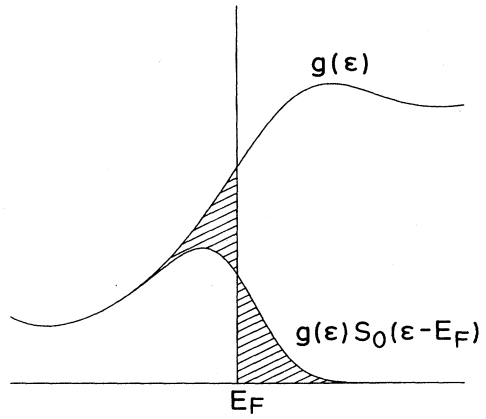
\includegraphics[height=1.1in,width=1.25in,viewport=0 0 530 500,clip]{Figures/MP_distribution.png}
	\caption{\textrm{A schematic density of states $g(\varepsilon)$ and function multiplied by a smooth distribution function.}}%
	\label{MP_distribution}
	%\hspace*{-10pt}
	\end{figure} 
}

\frame
{
\frametitle{$\vec k$~空间布点与积分}
	\textcolor{red}{简单分布函数}
		\begin{itemize}
			\item 
				\begin{figure}[h!]
					\begin{minipage}[t]{0.40\linewidth}
						\textrm{Fermi-Dirac~}分布函数$$f(\varepsilon)=\dfrac1{\mathrm{e}^{(\varepsilon-\mu)/kT}+1}$$ 
						其中$\mu$是化学势,$k$~是\textrm{Boltzmann}常数,$T$是温度参数
					\end{minipage}
				\hfill
					\begin{minipage}[t]{0.55\linewidth}
					\centering
					\vspace*{-0.35in}
					\hspace*{-0.5in}
					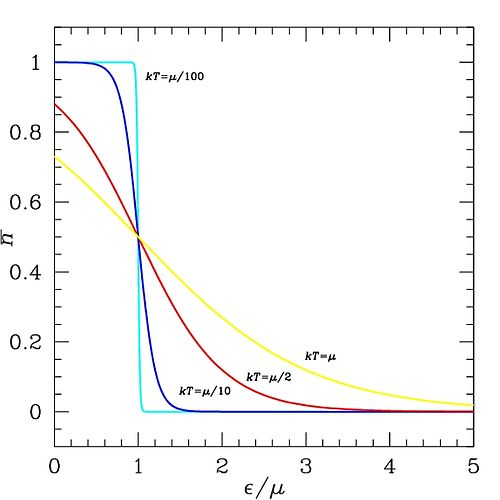
\includegraphics[height=1.0in,width=1.25in,viewport=0 0 530 500,clip]{Figures/Fermi-Dirac-distribution.jpg}
					\caption{\textrm{The Fermi-Dirac Distribution.}}%
					\label{Fermi-Dirac-distribution}
					\end{minipage}
					%\hspace*{-10pt}
				\end{figure} 
			\item 
				\begin{figure}[h!]
					\begin{minipage}[t]{0.40\linewidth}
						\textrm{Gaussian~}分布函数$$f(\varepsilon)=\dfrac1{\sigma\sqrt{2\pi}}\mathrm{e}^{-\frac{(\varepsilon-\mu)^2}{2\sigma^2}}$$
						其中$\mu$是化学势,$\sigma$是展宽参数
					\end{minipage}
				\hfill
					\begin{minipage}[t]{0.55\linewidth}
					\centering
					\vspace*{-0.35in}
					\hspace*{-0.5in}
					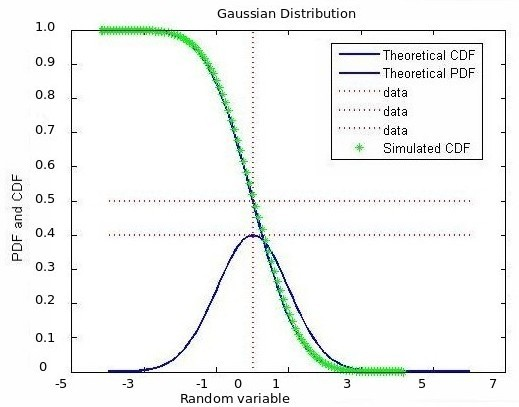
\includegraphics[height=1.0in,width=1.25in,viewport=0 0 530 500,clip]{Figures/Gaussian-distribution.jpg}
					\caption{\small \textrm{The Gaussian Distribution.}}%
					\label{Gaussian-distribution}
					\end{minipage}
					%\hspace*{-10pt}
				\end{figure} 
%			\item \textrm{Lorentz~}分布函数$$L(x)=\frac1{\pi}\frac{\frac12\Gamma}{(x-x_0)^2+\left(\frac12\Gamma\right)^2}$$
%				这里$x_0$是中心,$\Gamma$是展宽参数
		\end{itemize}
}

\frame
{
	\frametitle{\textrm{Monkhorst-Pack}布点方案}
	\textcolor{red}{特殊点方法}
\begin{figure}[h!]
\begin{minipage}[t]{0.52\linewidth}
	\textrm{Monkhorst-Pack}提出按如下简易方案划分\textrm{Brillouin-zone}\upcite{PRB13-5188_1976}:
			$$\boxed{u_r=\dfrac{(2r-q-1)}{2q}\quad(r=1,2,3,\cdots,q)}$$
			$q$是确定特殊点数目的某个整数
			\vspace{-0.1in}
			$$A_m(\vec k)=N_m^{-1/2}\sum_{|\vec R|=C_m}\mathrm{e}^{\mathrm{i}\vec k\cdot\vec R}$$
\end{minipage}
\hfill
\begin{minipage}[t]{0.42\linewidth}
\centering
%\hspace*{2pt}
\vspace*{-0.6in}
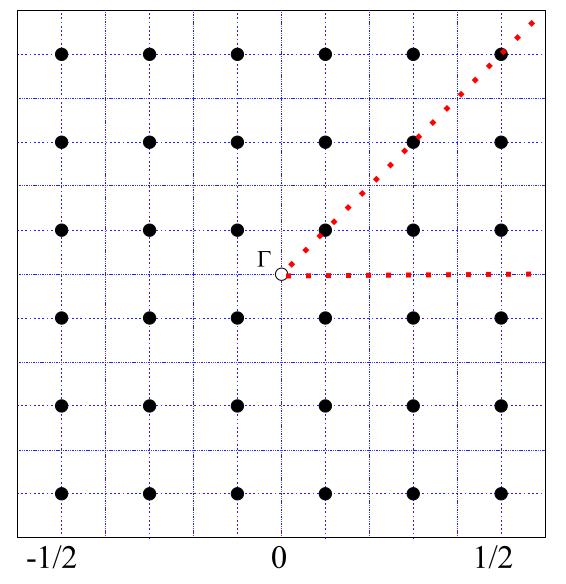
\includegraphics[height=1.5in,width=2.05in,viewport=-200 0 850 800,clip]{Figures/Special-points-MP.png}
\caption{\small \textrm{The generation of special $\vec k$-points in \textrm{Monkhorst-Pack} method.}}%
\label{Special-points-MP}
\end{minipage}
\end{figure} 
	
}

\frame
{
	\frametitle{逼近函数}
	利用\textrm{Hermite}~多项式的等式关系$$\frac{\mathrm d}{{\mathrm d}x}[H_n(x)\mathrm{e}^{-x^2}]=-H_{n+1}(x){\mathrm e}^{-x^2}$$
	\begin{figure}[h!]
		\begin{minipage}[t]{0.55\linewidth}
			\textrm{Methfessel-Paxton~}提出利用逼近函数提高积分精度\upcite{PRB40-3616_1989}
		\begin{displaymath}
			\begin{aligned}
				S_0(x)&=\frac12\left[1-\mathrm{erf}(x)\right]\\
				S_N(x)&=S_0(x)+\sum_{n=1}^NA_nH_{2n-1}(x)\mathrm{e}^{-x^2}
			\end{aligned}
		\end{displaymath}
		\textcolor{blue}{$S_0$对应于\textrm{Gaussian}分布函数}(类似\textrm{Fermi-Dirac}分布函数)
		\end{minipage}
		\hfill
		\begin{minipage}[t]{0.40\linewidth}
		\centering
		\vspace*{-0.8in}
%		\hspace*{0.5in}
		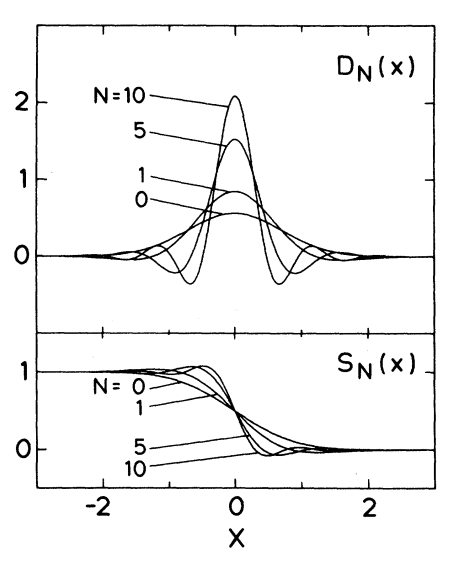
\includegraphics[height=2.0in,width=1.25in,viewport=0 0 530 800,clip]{Figures/MP_SN_DN.png}
		\caption{\textrm{Sucessive approximants to the $\delta$ function, $D_N$ and to the step function $S_N$.}}%
		\label{MP_SN_DN}
		%\hspace*{-10pt}
		\end{minipage}
	\end{figure} 
	\textrm{Methfessel-Paxton~}提出用更复杂的多项式函数$S_N$,引入变量$x=(\varepsilon-E_{\mathrm F})/W$,为了用函数$S_N(x)$逼近\textrm{Step~}函数$S(x)$,%,并要求$S_N$是平滑函数
}

\frame
{
\frametitle{四面体积分}
	\textcolor{red}{四面体方法\textrm{(Tetrahedron schemen)}}
	\begin{itemize}
		\item 四面体方法是一种线性插值方法,将\textrm{Brillouin-zone~}用体积相等的四面体填充,在每个四面体内部,被积函数$X_n(\vec k_j)$和能量$\varepsilon_n^{\vec k_j}$都随$\vec k$~点线性变化
		\item 一般来说,四面体方法对金属和导体的\textrm{Fermi~}面确定更可靠
		\item \textcolor{blue}{如何方便地确定每个$\vec k$~点的积分权重$w_n^{\vec k_i}$,精确、高效地完成\textrm{Brillouin-zone~}积分是$\vec k$~空间布点方案的主要研究内容}
	\end{itemize}
	\textrm{Bl\"ochl}提出了高效解决四面体生成和积分权重计算方法,参见文献\cite{PRB49-16233_1994}
}

\frame
{
	\frametitle{四面体积分权重}
\begin{figure}[h!]
\centering
\subfigure[\textrm{\small Arrangement of the different secant planes of constant energy in the method of tetrahedrons}]{
\label{Fig:Tetra-equal-ene}
\vspace*{-0.30in}
	\includegraphics[height=1.53in,width=2.00in,viewport=40 125 530 465,clip]{Figures/Tetra-equal-ene.eps}}
	\hfill
\subfigure[\textrm{\small Two-dimensional schematic illustration of the function $w_j(\vec k)$.}]{
\label{Fig:Submesh_Tetra}
\vspace*{-0.30in}
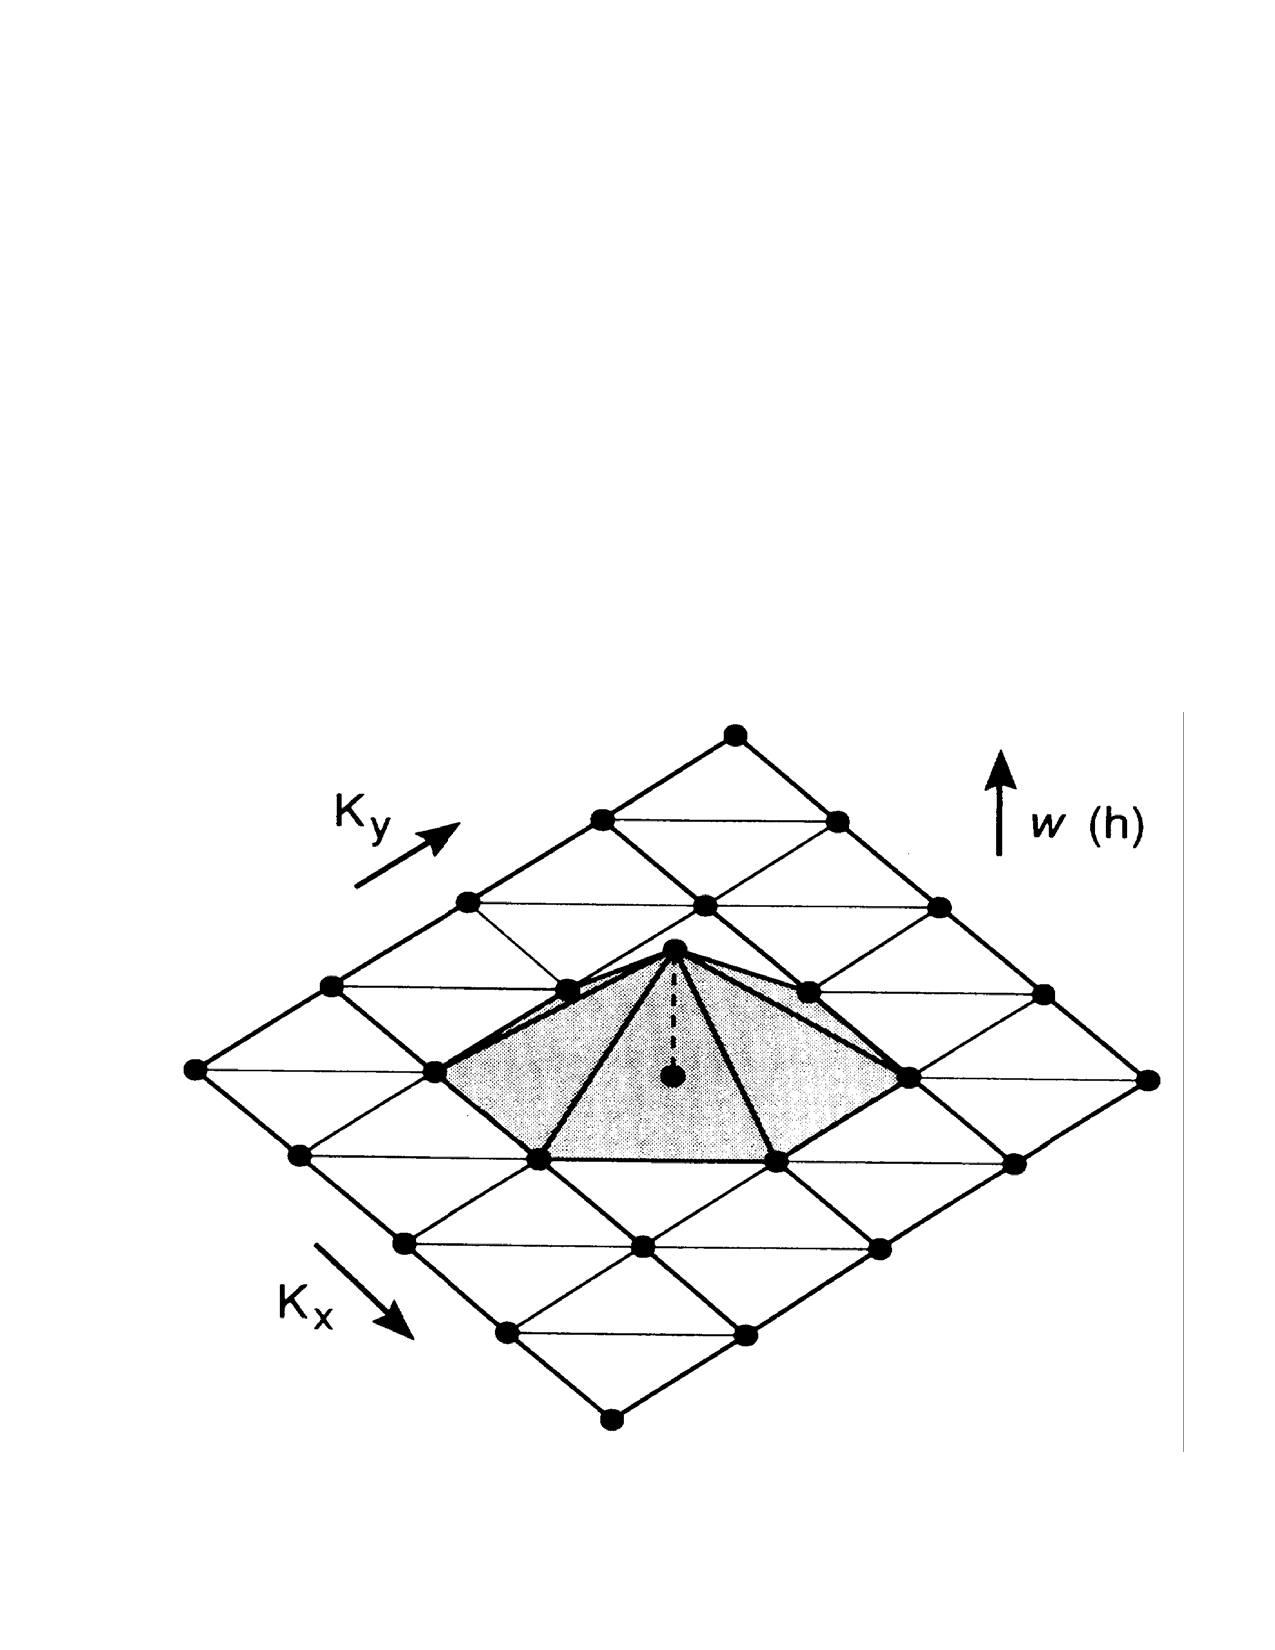
\includegraphics[height=1.75in,width=1.75in,viewport=0 30 565 505,clip]{Figures/dimen_Tetra.pdf}}
\end{figure}
\fontsize{9.2pt}{3.9pt}\selectfont{根据能量范围的不同,可以推导出不能能量区域内的积分权重的表达式,详见文献\cite{PRB49-16233_1994}的附录}
}

\frame
{
	\frametitle{四面体积分权重计算}
\begin{figure}[h!]
\begin{minipage}[t]{0.45\linewidth}
\centering
\includegraphics[height=1.25in,width=1.50in,viewport=15 15 250 190,clip]{Figures/Tetrahedron.eps}
\caption{\small Arrangement of the secant plane of constant energy in the method of tetrahedrons when $\varepsilon_0\leqslant\varepsilon_F\leqslant\varepsilon_1$.}%(与文献\cite{EPJB33-47_2003}图1对比)
\label{Fig:Tetrahedron}
\end{minipage}
\hfill
\begin{minipage}[t]{0.50\linewidth}
	\vspace*{-100pt}
	在每个四面体内,等能面$\varepsilon$的线性插值表示
		\begin{displaymath}
			\begin{aligned}
				\vec k_{10}(\varepsilon)=&\vec k_{10}\frac{\varepsilon-\varepsilon_0}{\varepsilon_1-\varepsilon_0}\\
				\vec k_{20}(\varepsilon)=&\vec k_{20}\frac{\varepsilon-\varepsilon_0}{\varepsilon_2-\varepsilon_0}\\
				\vec k_{30}(\varepsilon)=&\vec k_{30}\frac{\varepsilon-\varepsilon_0}{\varepsilon_3-\varepsilon_0}\\
			\vec k_0(\varepsilon)=&\vec k_0+a_1\vec k_{10}(\varepsilon)+a_2\vec k_{20}(\varepsilon)\\
			+&a_3\vec k_{30}(\varepsilon)
			\end{aligned}
		\end{displaymath}
		\hspace*{-15pt}引入矢量$g_{i0}$,满足$\vec g_{i0}\vec k_{j0}=\delta_{ij}$
\end{minipage}
\end{figure}
%\vspace*{-5pt}
		$$\varepsilon(\vec k)=\varepsilon_0+\sum_i^3(\varepsilon_i-\varepsilon_0)\vec g_{i0}(\vec k-\vec k_0)=\varepsilon_0+(\varepsilon-\varepsilon_0)(a_1+a_2+a_3)$$
%		根据条件$\varepsilon=\varepsilon_i(i=1,2,3)$确定系数
}

\frame
{
	\frametitle{四面体的生成}
%类似地,可以有四面体方法态数目(\textrm{number of states})、态密度(\textrm{Density of States, DOS})$D_T(\varepsilon_i)$的贡献表达式,具体可参见文献\cite{PRB49-16233_1994}。
	为了减少统计四面体的数目,可以先找出第一\textrm{Brillouin-zone}的不可约部分。但这一策略有副作用,\textcolor{red}{由于不可约部分的不规则性,其中的四面体划分几乎不可避免地要人工干预,不利于编程求解}\\\textrm{Bl\"ochl}提出一个解决方法:\\
\begin{enumerate}
	\item 利用\textrm{Monkhorst-Pack}方案\upcite{PRB13-5188_1976}首先在第一\textrm{Brillouin-zone}内生成等体积的平行六面体网格。
	\item 依次给每个点编号:
\begin{displaymath}
	\boxed{N=1+\dfrac{i-i_0}2+(n_1+1)\left[\dfrac{j-j_0}2+(n_2+1)\dfrac{k-k_0}2\right]}
\end{displaymath}
其中$i,j,k$分别是该$\vec k$~点沿倒格矢$\mathbf{b}_i(i=1,2,3)$的序数的二倍,$i_0,j_0,k_0$是\textrm{Monkhorst-Pack}方法中点的偏移量,有偏移则为1,否则为0。
\end{enumerate}
}

\frame
{
	\frametitle{四面体的生成}
\begin{enumerate}
	\setcounter{enumi}{2}
	\item 编号之后建立标识数组,其位置与该位置储存的元素值相同,例如,第一个位置存储“$1$”,第二个位置存储“$2$”,依次类推
	\item 然后从第一个位置开始,利用对称群的操作矩阵对每个点坐标作用,并与数组中其他点的坐标进行比较,如果彼此相同且后者的编号大于前者,即将后者的元素值改为前者\\\textcolor{blue}{对全部数组操作完毕,可以挑出所有不可约$\vec k$~点:\\只有当$\vec k_i$~为不可约$\vec k$~点时,其编号才与其存储位置相同}。
	\item 为了计算方便,可以对所有这些不可约$\vec k$~点按存储位置的顺序重新编号,即从“$1$”到“$\vec k_{\mathrm{irr}}(\max)$”。数组中的各个元素也相应的改为新的编号。这样整个第一\textrm{Brillouin-zone}中的点都可用不可约点标记。
\end{enumerate}
}

\frame
{
	\frametitle{四面体的生成}
\begin{figure}[h!]
\centering
\vspace*{-0.28in}
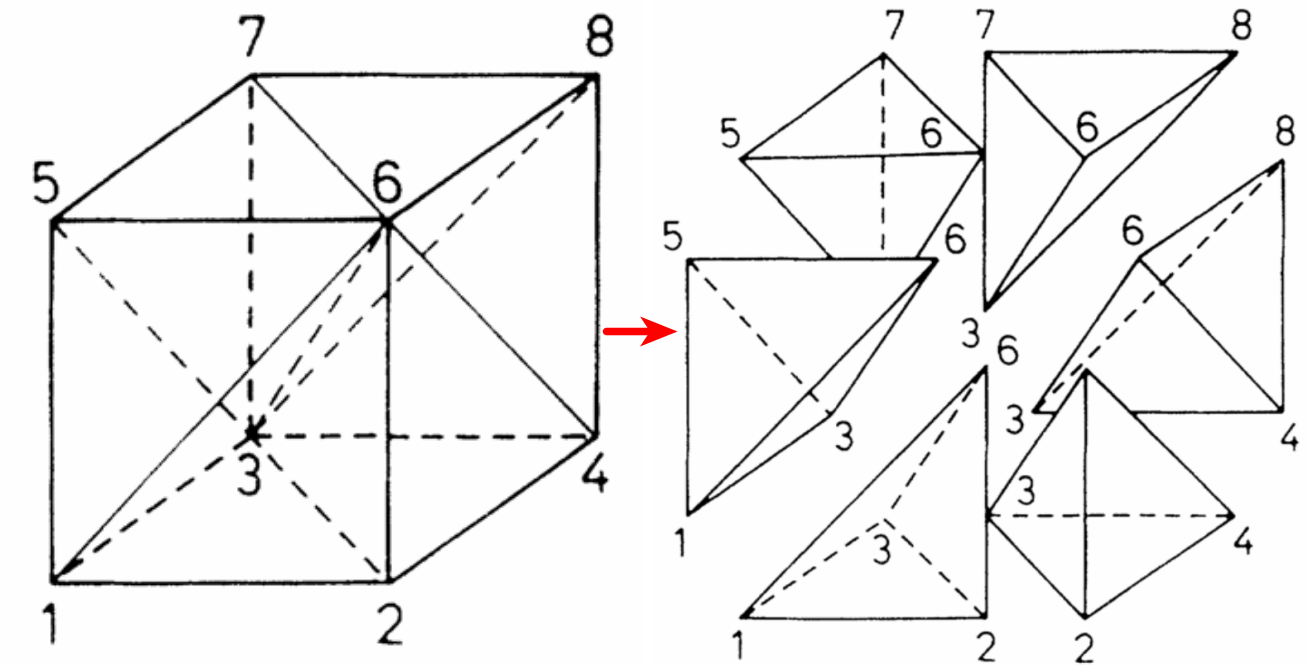
\includegraphics[height=1.25in,width=3.00in,viewport=0 0 1350 705,clip]{Figures/submesh_Tetra.png}
\caption{\small Breakup of a submesh cell into six tetrahedra.}%(与文献\cite{EPJB33-47_2003}图1对比)
\label{Fig:Submesh_Tetra}
\end{figure}
\fontsize{9.2pt}{3.9pt}\selectfont{对每个平行六面体重复上述过程,将第一\textrm{Brillouin-zone}划分为体积相等的若干四面体,每个四面体的顶点可用标识数组中的不可约点标记。将这四个顶点的标号按升序排列,可以方便地确定等价四面体(简并度)\\
这个过程保证了\textcolor{red}{只用不可约点上的信息进行整个第一\textrm{Brillouin}区的积分,无须考虑如何划定其不可约部分}\\
%上述过程可以避免Kleinman所说的计算误差,而且整个过程可以通过程序自动实现而无须人工干预。
上述过程可以避免计算误差,而且整个过程可以通过程序自动实现而无须人工干预}
}
%------------------------------------------------------------------------Reference----------------------------------------------------------------------------------------------
\begin{thebibliography}{99}
%-----------------------------------------------------------------------------------------------------------------------------------------------------------------------%
\frame
{
\frametitle{主要参考文献}
{\fontsize{7.2pt}{3.9pt}\selectfont{
	\bibitem{PRB59-1758_1999}\textrm{G. Kresse and D. Joubert \textit{Phys. Rev.} B, \textbf{59} (1999), 1758}
	\bibitem{Comp_Phys}\textrm{J. M. Thijssen. \textit{Computational Physics (2nd Edition)} (Cambridge University Press, Cambridge, England, 2007)}
        \bibitem{CMS6-15_1996}\textrm{G. Kresse and J. Furthm\"uller \textit{Comput. Mat. Sci.}, \textbf{6} (1996), 15}
	\bibitem{PRB54-11169_1996}\textrm{G. Kresse and J. Furthm\"uller \textit{Phys. Rev.} B, \textbf{54} (1996), 11169}
	\bibitem{VASP_UG}\textrm{G. Kresse, M. Marsman, and J. Furthm\"uller. \textit{VASP the GUIDE}. Computational Physics, Faculty of Physics, Universit\"at Wien, Austria (2012) \\\url{http://cms.mpi.univie.ac.at/VASP/}}
	\bibitem{Crelle30-51_1846}\textrm{C. G. Jacobi,\textbf{\"Uber ein leichtes Verfahren die in der Theorie der S\"acul\"arst\"orrungen vorkommenden Gleichungen numerisch aufzul\"osen}, \textit{Crelle's J.} \textbf{30} (1846), 51-94}
	\bibitem{PRB13-5188_1976}\textrm{H. J. Monkhorst and J. D. Pack \textit{Phys. Rev.} B, \textbf{13} (1976), 5188}
	\bibitem{PRB40-3616_1989}\textrm{M. Methfessel and A. T. Paxton \textit{Phys. Rev.} B, \textbf{40} (1989), 3616}
	\bibitem{PRB49-16233_1994}\textrm{P. E. Bl\"ochl, O. Jepsen and O. K. Andersen. \textit{Phys. Rev.} B, \textbf{49} (1994), 16233}
	\bibitem{Elect_Stru}\textrm{Richard. M. Martin. \textit{Electronic Structure: Basic Theory and Practical Methods} (Cambridge University Press, Cambridge, England, 2004)}
}}
}

%\frame
%{
%\frametitle{主要参考文献}
%{\small
%\bibitem{Singh_Book}\textrm{D. J. Singh. \textit{Plane Wave, PseudoPotential and the LAPW method} (Kluwer Academic, Boston,USA, 1994)}					%
%  \nocite{*}																				%
%}
%}
\end{thebibliography}

%-----------------------------------------------------------Beamer下不建议使用bib,因为涉及分页--------------------------------------------------------------------------%
%{\small
%\phantomsection\addcontentsline{toc}{section}{Bibliography}	 %直接调用\addcontentsline命令可能导致超链指向不准确,一般需要在之前调用一次\phantomsection命令加以修正	%
%\bibliography{Myref}																			%
%\bibliographystyle{mybib}																		%
%  \nocite{*}																				%
%}

%------------------------------------------------------------------------------------------------------------------------------------------------------------------------------%

%\end{thebibliography}

%-------------------------------------------------------------------------Thanks------------------------------------------------------------------------------------------------
%\section{致谢}
%\frame
%{
%\frametitle{致$\quad$谢}
%\begin{itemize}
%    \setlength{\itemsep}{20pt}
%  \item 感谢本团队高兴誉、吴泉生、宋红州等各位老师参与的讨论
%  \item 感谢莫所长、宋主任以及软件中心各位老师和同事
%  \item 感谢王崇愚先生的帮助
%\end{itemize}
%}

\logo{}									%不显示logo
\frame
{
\vskip 60 pt
%\hskip 10pt \textcolor{blue}{\Huge 感谢答辩委员会各位老师\,\textrm{!}}\\
\vskip 35 pt
\hskip 60pt \textcolor{blue}{\Huge 谢谢大家\:!}
%\vskip 15 pt
%\hskip 40pt \textcolor{blue}{\Huge \textrm{for your attention\:!}}
}

%-------------------------------------------------------------------------------------------------------------------------------------------------------------------------------

\clearpage
%\end{CJK*}
\end{document}
